%%%%%%%%%%%%%%%%%%%%%%%%%%%%%%%%%%%%%%%%%
% Masters/Doctoral Thesis 
% LaTeX Template
% Version 1.42 (19/1/14)
%
% This template has been downloaded from:
% http://www.latextemplates.com
%
% Original authors:
% Steven Gunn 
% http://users.ecs.soton.ac.uk/srg/softwaretools/document/templates/
% and
% Sunil Patel
% http://www.sunilpatel.co.uk/thesis-template/
%
% License:
% CC BY-NC-SA 3.0 (http://creativecommo\textit{•}ns.org/licenses/by-nc-sa/3.0/)
%
% Note:
% Make sure to edit document variables in the Thesis.cls file
%
%%%%%%%%%%%%%%%%%%%%%%%%%%%%%%%%%%%%%%%%%

%----------------------------------------------------------------------------------------
%	PACKAGES AND OTHER DOCUMENT CONFIGURATIONS
%----------------------------------------------------------------------------------------

\documentclass[11pt, a4paper]{Thesis} % Paper size, default font size and one-sided paper

\graphicspath{{Pictures/}} % Specifies the directory where pictures are stored

\usepackage{comment}
\usepackage{pdfpages}
\usepackage{hyperref} 
\usepackage{array}
\usepackage{graphicx}

\usepackage[square, numbers, comma, sort&compress]{natbib} % Use the natbib reference package - read up on this to edit the reference style; if you want text (e.g. Smith et al., 2012) for the in-text references (instead of numbers), remove 'numbers' 
\hypersetup{urlcolor=blue, colorlinks=true} % Colors hyperlinks in blue - change to black if annoying
\title{\ttitle} % Defines the thesis title - don't touch this

\let\cleardoublepage\clearpage

\usepackage{titlesec}
\titleformat{\chapter}[hang]
{\normalfont\huge\bfseries}{\chaptertitlename\ \thechapter:}{1em}{}
\titlespacing*{\chapter}{0cm}{-\topskip}{0pt}[0pt]
\titlespacing{\section}{0pt}{*0}{*0}
\titlespacing{\subsection}{0pt}{*0}{*0}
\titlespacing{\subsubsection}{0pt}{*0}{*0}

\begin{document}

\frontmatter % Use roman page numbering style (i, ii, iii, iv...) for the pre-content pages

\setstretch{1.5} % Line spacing of 1.5

% Define the page headers using the FancyHdr package and set up for one-sided printing
\fancyhead{} % Clears all page headers and footers
\rhead{\thepage} % Sets the right side header to show the page number
\lhead{} % Clears the left side page header

\pagestyle{fancy} % Finally, use the "fancy" page style to implement the FancyHdr headers

\newcommand{\HRule}{\rule{\linewidth}{0.5mm}} % New command to make the lines in the title page

% PDF meta-data
\hypersetup{pdftitle={\ttitle}}
\hypersetup{pdfsubject=\subjectname}
\hypersetup{pdfauthor=\authornames}
\hypersetup{pdfkeywords=\keywordnames}

%----------------------------------------------------------------------------------------
%	TITLE PAGE
%----------------------------------------------------------------------------------------

\begin{titlepage}
\begin{center}

\textsc{\LARGE \univname}\\[1.5cm] % University name
\textsc{\Large Final Year Project}\\[0.5cm] % Thesis 
\Large \textit{Mid Project Report}\\[0.5cm]

\HRule \\[0.4cm] % Horizontal line
{\huge \bfseries \ttitle}\\[0.4cm] % Thesis title
\HRule \\[1.5cm] % Horizontal line
 
\begin{minipage}{0.4\textwidth}
\begin{flushleft} \large
\emph{Author:}\\
\href{https://engineering.leeds.ac.uk/cgi-bin/sis/comp/ts/student.cgi?student=200542912}{\authornames} % Author name - remove the \href bracket to remove the link
\end{flushleft}
\end{minipage}
\begin{minipage}{0.4\textwidth}
\begin{flushright} \large
\emph{Supervisor:} \\
\href{https://www.engineering.leeds.ac.uk/people/faculty/staff/r.s.kwan}{\supname} % Supervisor name - remove the \href bracket to remove the link  
\end{flushright}
\end{minipage}\\[3cm]
 
\large \textit{A final year project report submitted in fulfilment of the requirements\\ for the degree of \degreename}\\[0.3cm] % University requirement text
\textit{in the}\\[0.4cm]
\deptname\\[2cm] % Research group name and department name
 
{\large \today}\\[4cm] % Date
%\includegraphics{Logo} % University/department logo - uncomment to place it
 
\vfill
\end{center}

\end{titlepage}

\begin{comment}
%----------------------------------------------------------------------------------------
%	QUOTATION PAGE\usepackage{comment}
%----------------------------------------------------------------------------------------

\pagestyle{empty} % No headers or footers for the following pages

\null\vfill % Add some space to move the quote down the page a bit

\textit{``Thanks to my solid academic training, today I can write hundreds of words on virtually any topic without possessing a shred of information, which is how I got a good job in journalism."}

\begin{flushright}
Dave Barry
\end{flushright}

\vfill\vfill\vfill\vfill\vfill\vfill\null % Add some space at the bottom to position the quote just right

\clearpage  Start a new page

\end{comment}
%----------------------------------------------------------------------------------------
%	ABSTRACT PAGE
%----------------------------------------------------------------------------------------

\addtotoc{Abstract} % Add the "Abstract" page entry to the Contents

\abstract{\addtocontents{toc}{\vspace{1em}} % Add a gap in the Contents, for aesthetics

This project aims to allow more communication with outpatients in regards to their appointments. It also aims to tackle various problems such as attendance, human opportunity costs and patient satisfaction. This will be achieved using emerging technology to bridge the current communication gap between patients and the scheduling systems used.

\clearpage % Start a new page

\begin{comment}
%----------------------------------------------------------------------------------------
%	ACKNOWLEDGEMENTS
%----------------------------------------------------------------------------------------

\setstretch{1.3} % Reset the line-spacing to 1.3 for body text (if it has changed)

\acknowledgements{\addtocontents{toc}{\vspace{1em}} % Add a gap in the Contents, for aesthetics

The acknowledgements and the people to thank go here, don't forget to include your project advisor\ldots
}
\clearpage % Start a new page

\end{comment}

%----------------------------------------------------------------------------------------
%	LIST OF CONTENTS/FIGURES/TABLES PAGES
%----------------------------------------------------------------------------------------

\pagestyle{fancy} % The page style headers have been "empty" all this time, now use the "fancy" headers as defined before to bring them back

\lhead{\emph{Contents}} % Set the left side page header to "Contents"
\tableofcontents % Write out the Table of Contents

\lhead{\emph{List of Figures}} % Set the left side page header to "List of Figures"
\listoffigures % Write out the List of Figures

\begin{comment}
\lhead{\emph{List of Tables}} % Set the left side page header to "List of Tables"
\listoftables % Write out the List of Tables
\end{comment}

%----------------------------------------------------------------------------------------
%	ABBREVIATIONS
%----------------------------------------------------------------------------------------

\clearpage % Start a new page

\setstretch{1.5} % Set the line spacing to 1.5, this makes the following tables easier to read

\lhead{\emph{Abbreviations}} % Set the left side page header to "Abbreviations"
\listofsymbols{ll} % Include a list of Abbreviations (a table of two columns)
{
\textbf{NHS} & \textbf{N}ational \textbf{H}ealth \textbf{S}ervice \\
\textbf{APP} & Software \textbf{APP}lication \\
\textbf{API} & \textbf{A}lication \textbf{P}rogramming \textbf{I}nterface \\
\textbf{MVC} & \textbf{M}odel \textbf{V}iew \textbf{C}ontroller \\
\textbf{XML} & \textbf{E}xtensible \textbf{M}arkup \textbf{L}anguage \\
\textbf{JSON} & \textbf{J}ava\textbf{S}cript \textbf{O}bject \textbf{N}otation language \\
\textbf{SQL} & \textbf{S}tructured \textbf{Q}uery \textbf{L}anguage \\
\textbf{LINQ} & \textbf{L}anguage \textbf{IN}tegrated \textbf{Q}uery\\
\textbf{ER} & \textbf{E}ntity \textbf{R}elationship\\
\textbf{GCM} & \textbf{G}oogle \textbf{C}loud \textbf{M}essaging\\
}

%----------------------------------------------------------------------------------------
%	THESIS CONTENT - CHAPTERS
%----------------------------------------------------------------------------------------

\mainmatter % Begin numeric (1,2,3...) page numbering

\pagestyle{fancy} % Return the page headers back to the "fancy" style

% Include the chapters of the thesis as separate files from the Chapters folder
% Uncomment the lines as you write the chapters

\setstretch{1.5}

% Chapter 1

\chapter{Project Overview} % Main chapter title

\label{Chapter1} % For referencing the chapter elsewhere, use \ref{Chapter1} 

\lhead{Chapter 1. \emph{Project Overview}} % This is for the header on each page - perhaps a shortened title

%----------------------------------------------------------------------------------------

\section{Project Aim}

The aim of this project is to develop a system that allows more communication with outpatients in regards to their appointments, in an attempt to: 

\begin{itemize}
  \item reduce the amount of resources wasted in the event of no-shows and cancellations
  \item reducing the human cost that is required to manage appointments
  \item increase the user experience when making and managing an appointment
\end{itemize}

This project will not aim to implement any scheduling algorithms, but rather create a system that will support current algorithms and possibly shape future algorithms. For this project, I will use a preordained scenario to show off the different features of the system.

It will also not aim to replace the current scheduling system entirely, but act as an alternative to allow willing patients more direct control and easier access to information regarding their appointments. 

%----------------------------------------------------------------------------------------

\section{Objectives}

The objectives of this project is to:

\begin{itemize}
  \item Collect relevant background data about the problem domain
  \item Identify requirements necessary to address the problem
  \item Design a server-client system that implements these requirements
  \item Prototype a Server that communicates directly with multiple patients and a predetermined scheduling algorithm
  \item Prototype a Client Application (Smart-phone Application) that allows patients to interface with the server
  \item Test the systems functionality based on usability and performance
  \item Evaluate the success of the system in regards to improving user satisfaction, reducing human management resources and reducing appointment wastage
\end{itemize}

%----------------------------------------------------------------------------------------

\section{Minimum Requirements}

The minimum requirements of this project is to:

\begin{itemize}
	\item A working prototype smart-phone application that:
	\begin{itemize}
		\item Connects to a prototype server
		\item Allows the user to view information on their scheduled medical appointments
		\item Gives the user information such as location and map instructions, doctor's name, any perquisite tasks the user must undertake prior to the appointment
		\item Reminds the user about the appointment
		\item Receives appointment updates from the server
	\end{itemize}
	\item A working prototype server application that:
		\begin{itemize}
			\item Connects to multiple clients
			\item Interfaces with a dumb appointment scheduler
			\item Notifies clients of changes to the schedule
			\item Uses client information to optimise the scheduling process
			\item Offers cancelled appointments to other clients
		\end{itemize}
\end{itemize}

%----------------------------------------------------------------------------------------

\section{Extensions}

The possible extensions are:

\begin{itemize}
	\item TODO Put some of tasks from min requirements here
\end{itemize}

%----------------------------------------------------------------------------------------

\section{Deliverables}

The deliverables are:

\begin{itemize}
	\item Server application
	\item Client application
	\item Report and evaluation results
\end{itemize}

%----------------------------------------------------------------------------------------

\section{Relevance to Degree Modules}

This project uses knowledge and techniques gained in modules studied as part of my Computer Science degree. The most relevant modules are typically 'Software Systems Engineering', 'Distributed Systems', 'User Adaptive Systems' and 'Human Computer Interaction'.

%----------------------------------------------------------------------------------------
% Chapter Template

\chapter{Problem Description and Background Research} % Main chapter title

\label{Chapter2} % Change X to a consecutive number; for referencing this chapter elsewhere, use \ref{ChapterX}

\lhead{Chapter 2. \emph{Problem Description and Background Research}} % Change X to a consecutive number; this is for the header on each page - perhaps a shortened title

%----------------------------------------------------------------------------------------

\section{Problem Description}

Medical appointment scheduling is a complex problem; patients often come with different backgrounds and personal schedules, requiring different treatment and different urgency, some even requiring support in getting to the appointments. Patients sometimes have a need to cancel their appointments or simply do not turn up, which can lead to a waste in resources if the appointment slot is not then assigned to another patient. Often, sessions can overrun, requiring more time per patient than is estimated, and so the following appointments are delayed. Clinics also reschedule appointments regularly, as new patients requiring urgent medical attention become a higher priority. This results in appointments being dynamic, often the time and date of the actual appointment is different from what was originally planned.

Dynamic scheduling leads to many issues. The problem of scheduling appointments becomes far more complex, which in turn requires more staff resources to manage the appointments.

Communication also becomes a problem, as patients need to be informed about all changes to the original schedule. Often, this results in a lower patient satisfaction and a higher chance of appointment cancellations.

These often contribute to longer waiting times and a lack of patient knowledge about their appointments, which can make no-shows and further last-minute cancellations more frequent. Often the clinic will not find a patient to take the free appointment slot, and these resources are wasted.

\subsection{Wasted Resources}

Many resources are wasted through appointment no-shows and cancellations. Research shows that the longer a patient must wait between making the appointment and the actual appointment date, the more likely it is that they will either cancel or not turn up\cite{Gallucci}. Although we can see that there is a relationship between the length of time that a patient must wait for an appointment and the cancellation risk, it is important to understand why.

The most common reasons why patients do not show up was collected through patient questionnaires as can be seen in the figure below.

\begin{figure}[htbp]
	\centering
		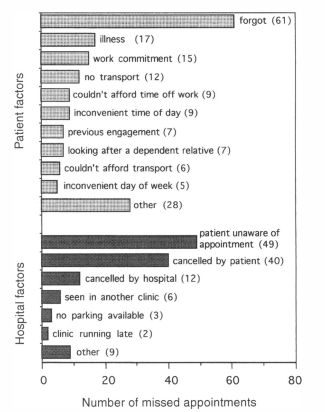
\includegraphics{Figures/MissedAppointmentsStoneEtAl.png}
		\rule{35em}{0.5pt}
	\caption[Factors contributing to non-attendance according to a patient questionaire - \cite{Stone}]{Factors contributing to non-attendance according to a patient questionaire - \cite{Stone}}
	\label{fig:NonAttendance}
\end{figure}

This shows that the most common factor is either that the patient forgot or that they were improperly informed by the clinic.

\subsubsection{Patient No-Shows}

Patient no-shows (or non-attendance at outpatient clinics) are a big problem in appointment scheduling and is one of the largest contributors to wasted resources in the NHS. It is estimated  that the financial cost of missed appointments contributes to a loss of £360 million per year\cite{Stone}. Besides the financial costs, it also increases waiting times as that patient must be rescheduled for another appointment, effectively doubling the required resources per patient. 

Because the most common factor contributing to no-shows is the patient forgetting to attend the appointment, it suggests a reminder system could be used effectively to reduce these numbers. Research has shown that telephone and postal reminders can help, but have not proved to be cost effective in the past\cite{Mann}. However, through recently emerging online devices and 'smart' technology, it is possible to provide a low-cost solution to this problem.

Another factor that can encourage non-attendance can be a lack of information known about the appointment. This can introduce a level of uncertainty within the patient, such as knowledge on how to get to their appointment, or  fear about the dangerous/embarrassing factors involved in the appointment\cite{Frankel}.

Research shows that the population that miss appointments are increasingly of a young demographic. Often they fail to understand why the appointments are important, and specifically why it is important to cancel the appointment rather than just not turn up.

Patients have given several reasons for no-shows in studies and questionnaires\cite{Lacy}:

\begin{itemize}
	\item can't get time off work
	\item child-care
	\item lack of transportation or cost
	\item patient felt better or felt too worse to attend the appointment
\end{itemize}

For all these reasons, the no-show is preventable simply by increasing communication with the patient and allowing them either more information about the appointment or making it easier for them to either cancel/reschedule.

\subsubsection{Cancellations}

Often, clinics are required to cancel an outpatients appointment for a variety of reasons, usually due to a lack of resources such as staff or equipment.

Staff time is then wasted getting contact information for the patient and informing them of the cancellation. Time must also be spent corresponding with the patient and agreeing on a suitable replacement appointment.

If cancellations 'occur at the last minute', often the patient is not informed until they reach the hospital. This is often due to the clinic not wanting to bother wasting resources reaching the patient when it is unlikely that they will get a hold of them (the patient may already be in transit or indisposed). This leads to a lower overall user satisfaction as the patient wastes a trip to the hospital, only to find that they no longer have an appointment.

Although cancellations are not ideal, they are better than no-shows in that it is possible for the appointment to be offered to another patient. In some cases however, this is not attempted due to it being too costly and the additional complexity involved in the scheduling process.

By increasing communication with patients through emerging smart technology, it may be possible for these appointments to be quickly rescheduled whilst avoiding the additional costs, even for 'last-minute' cancellations.

\subsubsection{Managing Appointments}

Managing appointments is costly and a large proportion of the work is carried out by individual staff members, rather than an automated system. Several issues arise with this process:

\begin{itemize}
	\item Appointments can only be managed within office hours (typically 9am - 5pm), however this depends on the clinic
	\item Patients can only make appointments over the phone and frequently have to queue to speak to a staff member
	\item Large proportions of staff members must be allocated to the appointments procedure which could be allocated elsewhere
	\item State of the system means that it is hard to analyse and therefore adapt to high demand
	
\end{itemize}

When making appointments, the patient is required to do so either in person or over the phone. This can only occur within office hours, which can conflict with the patients career or personal schedule, leading to a lower user satisfaction. Often patients will have to queue in order to speak to a staff member. When the patient is finally connected, there isn't time for the patient to explain their personal schedule and discuss conflicts, resulting in less user choice and flexibility.

The appointment system in many areas is also very labour-intensive, carried out by individual receptionists using spreadsheets and paper based systems\cite{ApointProcWebsite}. This means that it is often very hard to analyse capacity and demand, identifying bottlenecks or methods to improve them and also makes it very hard to integrate with interactive technology such as smart phone devices and online appointments. Whilst some online systems do exist\cite{C&BWebsite}, they are time consuming, have poor functionality and tend to be only available on few devices\cite{C&BFailure}. 

These problems can be improved by creating an interactive online system that works on many devices. It could not replace the current system entirely, because not all patients will have internet access or smart-devices, but it would provide benefits to patients with internet access such as:

\begin{itemize}
	\item Easier accessibility to making appointments
	\item Possibly offer more appointment flexibility to the patient
	\item More information about the appointment
	\item Relieve demand on the staff that manage the system
	\item More analysis of appointment trends and offer insights into improvement
\end{itemize}

\subsection{Patient Satisfaction and Experience}

Maintaining a high patient satisfaction is the primary goal in appointment scheduling, ultimately because keeping the patients happy leads to less cancellations and less no-shows. This is not an easy task because the demand on the healthcare system is so great, and it is typically faced with many challenges.

\subsubsection{Patient Requirements}

Patients are given a level of responsibility that some may not be used to. For a general outpatient appointment, the NHS requires the patient to do a number of tasks to prepare for the appointment \cite{OutpatientApointWebsite}:

\begin{itemize}
  \item may be required not to eat/drink before the appointment
  \item may be required to bring samples of urine/stool or medicines
  \item may need to bring previous test results
  \item may need to take certain medicines at a certain time period prior to the appointment
  \item should bring maps and other information required for getting to their appointment
\end{itemize}

It has been seen that in previous research conducted on day surgery outpatients, the most likely cause of preventable appointment cancellations (5\% of day surgery appointments) was due to inadequate preparation \cite{Macarthur}. This shows that a large amount of patient cancellations occur simply because patients are expected to find out information about their appointment, transport options and other relevant factors.

\subsubsection{Waiting times}

Another factor that lowers patient satisfaction are waiting times that can occur when the schedule is either running late due to overrunning appointments, or when patients are grouped into time slots.

Patients are frequently grouped together into time slots to simplify the scheduling process (i.e the clinic will expect to have 10 appointments in one hour, so they ask all 10 patients to come at the same time and the appointments occur on a first come first serve basis).

Research suggests that because patients spend increasingly lengthy amounts of time waiting in the clinic for their appointment to start, they feel increasingly amounts of disrespect \cite{Lacy}. This is due to patients being 'left in the dark', with no indication on why their appointment is delayed and why they have to wait.

Through on-line applications and smart devices, we can inform patients about information related to their appointments, any disruptions in the regular service (waiting delays) and a more interactive system that would make the patient feel less disrespect. We can also provide transport information, reminders on when they have to leave and any perquisite requirements that the patient must undertake before leaving for their appointment (such as take medication or bring test results).

%----------------------------------------------------------------------------------------

\section{Choose and Book - An existing online medical appointment service}

An NHS service 'Choose and Book' was launched in 2006, aimed at providing patients with more choice through online appointments\cite{Walford}.

This system is similar to the project area in that it allows patients to create online outpatient appointments, having a choice over which clinic they go to and when they the appointment is booked for.

However, an independent survey of patient's experience using the service in 2008 showed that patients did not receive the degree of choice that the service was designed to deliver\cite{Green}. It has also been widely criticised as being time consuming, over complicated and . An article in 2012\cite{C&BFailure} shows that the system's popularity is diminishing.

Besides the clear flaws in the system such as ease of use and failing to offer more choice, it also fails to target significant areas of the problem description, such as electronic reminders, recycling unused appointments and general appointment information.

%----------------------------------------------------------------------------------------

\section{Mobile Applications and Smart Devices}

Emerging 'smart' technology allows service providers to remain connected to users with almost no down time.

%----------------------------------------------------------------------------------------

\section{Conclusion}

Attempts have been made in the past to simplify the appointment management process and take it online, however they fail to hit all of the objectives simply because the platforms were not ready. As smart-devices and their many applications are becoming increasingly popular, it opens up a new gateway to communicate directly with patients and receive quick response times. This makes it much easier to create a dynamic appointment schedule whilst maintaining a high user satisfaction level.

This project will therefore focus on improving the communication and interactivity between patients and the appointment scheduling system; so that more information is available to the patient, there is more chance of reusing free appointment slots, and less staff resources are used in managing appointments so they can be allocated to other areas.

The project will also look at making the appointment creation and rescheduling process easier for both patients and staff, requiring less management resources and offering more platform choices and flexibility. 
% Chapter Template

\chapter{Problem Description and Background Research} % Main chapter title

\label{Chapter3} % Change X to a consecutive number; for referencing this chapter elsewhere, use \ref{ChapterX}

\lhead{Chapter 3. \emph{Problem Description and Background Research}} % Change X to a consecutive number; this is for the header on each page - perhaps a shortened title

%----------------------------------------------------------------------------------------

\section{Problem Description}

Medical appointment scheduling is a complex problem; patients often come with different backgrounds and personal schedules, requiring different treatment and different urgency, some even requiring support in getting to the appointments. Patients sometimes have a need to cancel their appointments or simply do not turn up, which can lead to a waste in resources if the appointment slot is not then assigned to another patient. Often, sessions can overrun, requiring more time per patient than is estimated, and so the following appointments are delayed. Clinics also reschedule appointments regularly, as new patients requiring urgent medical attention become a higher priority. This results in appointments being dynamic, often the time and date of the actual appointment is different from what was originally planned.

Dynamic scheduling leads to many issues. The problem of scheduling appointments becomes far more complex, which in turn requires more staff resources to manage the appointments.

Communication also becomes a problem, as patients need to be informed about all changes to the original schedule. Often, this results in a lower patient satisfaction and a higher chance of appointment cancellations.

These often contribute to longer waiting times and a lack of patient knowledge about their appointments, which can make no-shows and further last-minute cancellations more frequent. Often the clinic will not find a patient to take the free appointment slot, and these resources are wasted.

\subsection{Wasted Resources}

Many resources are wasted through appointment no-shows and cancellations. Research shows that the longer a patient must wait between making the appointment and the actual appointment date, the more likely it is that they will either cancel or not turn up\cite{Gallucci}. Although we can see that there is a relationship between the length of time that a patient must wait for an appointment and the cancellation risk, it is important to understand why.

The most common reasons why patients do not show up was collected through patient questionnaires as can be seen in the figure below.

\begin{figure}[htbp]
	\centering
		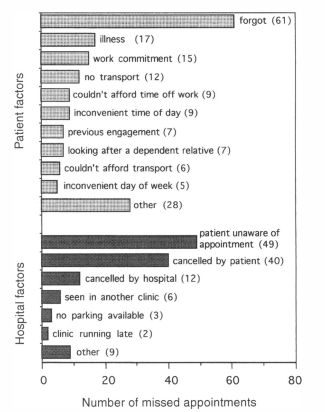
\includegraphics[width=10cm,height=10cm,keepaspectratio]{Figures/MissedAppointmentsStoneEtAl.png}
		\rule{35em}{0.5pt}
	\caption[Factors contributing to non-attendance according to a patient questionaire - \cite{Stone}]{Factors contributing to non-attendance according to a patient questionaire - \cite{Stone}}
	\label{fig:NonAttendance}
\end{figure}

This shows that the most common factor is either that the patient forgot or that they were improperly informed by the clinic.

\subsubsection{Patient No-Shows}

Patient no-shows (or non-attendance at outpatient clinics) are a big problem in appointment scheduling and is one of the largest contributors to wasted resources in the NHS. It is estimated  that the financial cost of missed appointments contributes to a loss of £360 million per year\cite{Stone}. Besides the financial costs, it also increases waiting times as that patient must be rescheduled for another appointment, effectively doubling the required resources per patient. 

Because the most common factor contributing to no-shows is the patient forgetting to attend the appointment, it suggests a reminder system could be used effectively to reduce these numbers. Research has shown that telephone and postal reminders can help, but have not proved to be cost effective in the past\cite{Mann}. However, through recently emerging online devices and 'smart' technology, it is possible to provide a low-cost solution to this problem.

Another factor that can encourage non-attendance can be a lack of information known about the appointment. This can introduce a level of uncertainty within the patient, such as knowledge on how to get to their appointment, or  fear about the dangerous/embarrassing factors involved in the appointment\cite{Frankel}.

Research shows that the population that miss appointments are increasingly of a young demographic. Often they fail to understand why the appointments are important, and specifically why it is important to cancel the appointment rather than just not turn up.

Patients have given several reasons for no-shows in studies and questionnaires\cite{Lacy}:

\begin{itemize}
	\item can't get time off work
	\item child-care
	\item lack of transportation or cost
	\item patient felt better or felt too worse to attend the appointment
\end{itemize}

For all these reasons, the no-show is preventable simply by increasing communication with the patient and allowing them either more information about the appointment or making it easier for them to either cancel/reschedule.

\subsubsection{Cancellations}

Often, clinics are required to cancel an outpatients appointment for a variety of reasons, usually due to a lack of resources such as staff or equipment.

Staff time is then wasted getting contact information for the patient and informing them of the cancellation. Time must also be spent corresponding with the patient and agreeing on a suitable replacement appointment.

If cancellations 'occur at the last minute', often the patient is not informed until they reach the hospital. This is often due to the clinic not wanting to bother wasting resources reaching the patient when it is unlikely that they will get a hold of them (the patient may already be in transit or indisposed). This leads to a lower overall user satisfaction as the patient wastes a trip to the hospital, only to find that they no longer have an appointment.

Although cancellations are not ideal, they are better than no-shows in that it is possible for the appointment to be offered to another patient. In some cases however, this is not attempted due to it being too costly and the additional complexity involved in the scheduling process.

By increasing communication with patients through emerging smart technology, it may be possible for these appointments to be quickly rescheduled whilst avoiding the additional costs, even for 'last-minute' cancellations.

\subsubsection{Managing Appointments}

Managing appointments is costly and a large proportion of the work is carried out by individual staff members, rather than an automated system. Several issues arise with this process:

\begin{itemize}
	\item Appointments can only be managed within office hours (typically 9am - 5pm), however this depends on the clinic
	\item Patients can only make appointments over the phone and frequently have to queue to speak to a staff member
	\item Large proportions of staff members must be allocated to the appointments procedure which could be allocated elsewhere
	\item State of the system means that it is hard to analyse and therefore adapt to high demand
	
\end{itemize}

When making appointments, the patient is required to do so either in person or over the phone. This can only occur within office hours, which can conflict with the patients career or personal schedule, leading to a lower user satisfaction. Often patients will have to queue in order to speak to a staff member. When the patient is finally connected, there isn't time for the patient to explain their personal schedule and discuss conflicts, resulting in less user choice and flexibility.

The appointment system in many areas is also very labour-intensive, carried out by individual receptionists using spreadsheets and paper based systems\cite{ApointProcWebsite}. This means that it is often very hard to analyse capacity and demand, identifying bottlenecks or methods to improve them and also makes it very hard to integrate with interactive technology such as smart phone devices and online appointments. Whilst some online systems do exist\cite{C&BWebsite}, they are time consuming, have poor functionality and tend to be only available on few devices\cite{C&BFailure}. 

These problems can be improved by creating an interactive online system that works on many devices. It could not replace the current system entirely, because not all patients will have internet access or smart-devices, but it would provide benefits to patients with internet access such as:

\begin{itemize}
	\item Easier accessibility to making appointments
	\item Possibly offer more appointment flexibility to the patient
	\item More information about the appointment
	\item Relieve demand on the staff that manage the system
	\item More analysis of appointment trends and offer insights into improvement
\end{itemize}

\subsection{Patient Satisfaction and Experience}

Maintaining a high patient satisfaction is the primary goal in appointment scheduling, ultimately because keeping the patients happy leads to less cancellations and less no-shows. This is not an easy task because the demand on the healthcare system is so great, and it is typically faced with many challenges.

\subsubsection{Patient Requirements}

Patients are given a level of responsibility that some may not be used to. For a general outpatient appointment, the NHS requires the patient to do a number of tasks to prepare for the appointment \cite{OutpatientApointWebsite}:

\begin{itemize}
  \item may be required not to eat/drink before the appointment
  \item may be required to bring samples of urine/stool or medicines
  \item may need to bring previous test results
  \item may need to take certain medicines at a certain time period prior to the appointment
  \item should bring maps and other information required for getting to their appointment
\end{itemize}

It has been seen that in previous research conducted on day surgery outpatients, the most likely cause of preventable appointment cancellations (5\% of day surgery appointments) was due to inadequate preparation \cite{Macarthur}. This shows that a large amount of patient cancellations occur simply because patients are expected to find out information about their appointment, transport options and other relevant factors.

\subsubsection{Waiting times}

Another factor that lowers patient satisfaction are waiting times that can occur when the schedule is either running late due to overrunning appointments, or when patients are grouped into time slots.

Patients are frequently grouped together into time slots to simplify the scheduling process (i.e the clinic will expect to have 10 appointments in one hour, so they ask all 10 patients to come at the same time and the appointments occur on a first come first serve basis).

Research suggests that because patients spend increasingly lengthy amounts of time waiting in the clinic for their appointment to start, they feel increasingly amounts of disrespect \cite{Lacy}. This is due to patients being 'left in the dark', with no indication on why their appointment is delayed and why they have to wait.

Through on-line applications and smart devices, we can inform patients about information related to their appointments, any disruptions in the regular service (waiting delays) and a more interactive system that would make the patient feel less disrespect. We will also be able to offer sooner appointments to patients as cancellations occur, which should reduce the waiting times overall.

We can also provide transport information, reminders on when they have to leave and any perquisite requirements that the patient must undertake before leaving for their appointment (such as take medication or bring test results), reducing the likelihood of cancellations and no-shows as the patient is better prepared..

\subsubsection{Patient Participation}

Patient participation is no longer just a goal set by medical commissioners, but a legal obligation. The Health and Social Care Act 2012\cite{HSCA2012} introduced legislation that enables patients(and carers) to participate in the planning, managing and making decisions
about their care and treatment.

The aim of this project targets this participation, engaging patients to have more control and access over their medical care. This system also has the ability to deliver personalised care plans to patients, which will increase the overall patient satisfaction.

Although this system does require patients to have access to the internet and know how to use it, patients without internet in today's world is an increasingly small demographic. The NHS are also launching a program to help disadvantaged people learn how to access the internet and use medical services \cite{timKelsey}, to try and combat these issues. 

%----------------------------------------------------------------------------------------

\section{Choose and Book - An existing online medical appointment service}

An NHS service 'Choose and Book' was launched in 2006, aimed at providing patients with more choice through online appointments\cite{Walford}.

This system is similar to the project area in that it allows patients to create online outpatient appointments, having a choice over which clinic they go to and when they the appointment is booked for.

However, an independent survey of patient's experience using the service in 2008 showed that patients did not receive the degree of choice that the service was designed to deliver\cite{Green}. It has also been widely criticised as being time consuming, over complicated and . An article in 2012\cite{C&BFailure} shows that the system's popularity is diminishing.

Besides the clear flaws in the system such as ease of use and failing to offer more choice, it also fails to target significant areas of the problem description, such as electronic reminders, recycling unused appointments and general appointment information.

%----------------------------------------------------------------------------------------

\section{Conclusion}

Attempts have been made in the past to simplify the appointment management process and take it online, however they fail to hit all of the objectives simply because the platforms were not ready. As smart-devices and their many applications are becoming increasingly popular, it opens up a new gateway to communicate directly with patients and receive quick response times. This makes it much easier to create a dynamic appointment schedule whilst maintaining a high user satisfaction level.

This project will therefore focus on improving the communication and interactivity between patients and the appointment scheduling system; so that more information is available to the patient, there is more chance of reusing free appointment slots, and less staff resources are used in managing appointments so they can be allocated to other areas.

The project will also look at making the appointment creation and rescheduling process easier for both patients and staff, requiring less management resources and offering more platform choices and flexibility.
% Chapter Template

\chapter{Design and Development} % Main chapter title

\label{Chapter4} % Change X to a consecutive number; for referencing this chapter elsewhere, use \ref{ChapterX}

\lhead{Chapter 4. \emph{Design and Development}} % Change X to a consecutive number; this is for the header on each page - perhaps a shortened title

%----------------------------------------------------------------------------------------


%---------------------------------------------------------------------------------------- 
% Chapter Template

\chapter{Implementation} % Main chapter title

\label{Chapter5} % Change X to a consecutive number; for referencing this chapter elsewhere, use \ref{ChapterX}

\lhead{Chapter 5. \emph{Implementation}} % Change X to a consecutive number; this is for the header on each page - perhaps a shortened title

%----------------------------------------------------------------------------------------

\section{Introduction}

This chapter will discuss in detail, the implementation of the proposed Android client application, and the server application that accompanies it.

With the system already designed out and with a list of set features, I started exploring various coding patterns I could use to implement my design.

\subsection{Architecture and Design Patterns}

Design patterns are reusable solutions to commonly occurring problems in software design. The use of tried and tested design patterns is important in software because it stops programmers from making the same mistakes, and also speeds up development time as you no longer need to 'reinvent the wheel' with every software engineering project.

Picking the correct design pattern for the problem can prove troublesome, and choosing the wrong ones can lead to inefficient solutions, such as unnecessary duplication of code.

For this project, 'MVC' was used heavily in both the client and server side application.

\subsubsection{Model-View-Controller (MVC)}

Model-View-Controller is a well known software design pattern for implementing user interfaces. The design follows three interconnected parts:

\begin{itemize}
	\item Model - holds the application data, and logic  for accessing and manipulating this data.
	\item View - holds logic that displays the aesthetic view to the user. It can also contain mechanisms of receiving user input and passing that input along to it's controller.
	\item Controller - holds controller logic that accesses data from a model and passes it to a view. It can also update a models state with new information, and update the view as the model is updated.
\end{itemize}

Figure \ref{fig:mvc} shows the MVC architecture.

\begin{figure}[htbp]
	\centering
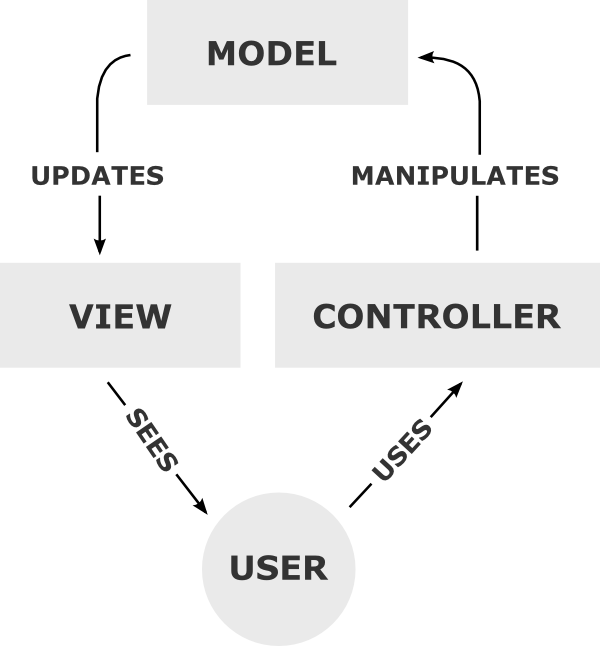
\includegraphics[width=\textwidth,height=\textheight,keepaspectratio]{Figures/MVC.png}	
		\rule{35em}{0.5pt}
	\caption[Model View Controller Diagram - \cite{wikiMVC}]{Model View Controller Diagram - \cite{wikiMVC}}
	\label{fig:mvc}
\end{figure}

The server application makes heavy use of certain aspects of MVC. Models are created for data storage and the transport of the objects from server to client. Controllers are also created to design restful web requests that the client can use to request the data models remotely. Views are not used in the project because no user interface is required for the web server.

The Android client application also uses this pattern, with the controllers requesting data from the remote server, using models to formulate the data into the right structure, and displaying the data in views.

\subsubsection{Component Pattern}

The component pattern is also used in the client application. The business logic is decoupled into separate components. A component is a typical manager class with helper functions that can be accessed anywhere in the applications code.

This allows the Android views to access different components and their functionality easily through a component manager.

\section{Project Setup}

A difficult part of the implementation was the development of both the client and the server at the same time, where features of the client are dependant on features of the server and vice versa.

For example, I could not implement the appointment information features of the client application until the server was able to send that information to it. I was also not able to test certain features of the server until the client had implemented ways of authenticating and sending the requests that the server would respond to.

\subsection{Emulating Requests}

To solve this problem, I used a tool called Postman to emulate the client requests to the server. 

Postman is a simple web application that allows you to design RESTful web requests very easily and send them to a server. By doing this, I was able to design and test the requests I needed easily.

This meant I could focus solely on implementing the basic server features without having to develop the Android application alongside it. I later found that this was also an invaluable method of testing server features when problems occurred.

\begin{figure}[htbp]
	\centering
		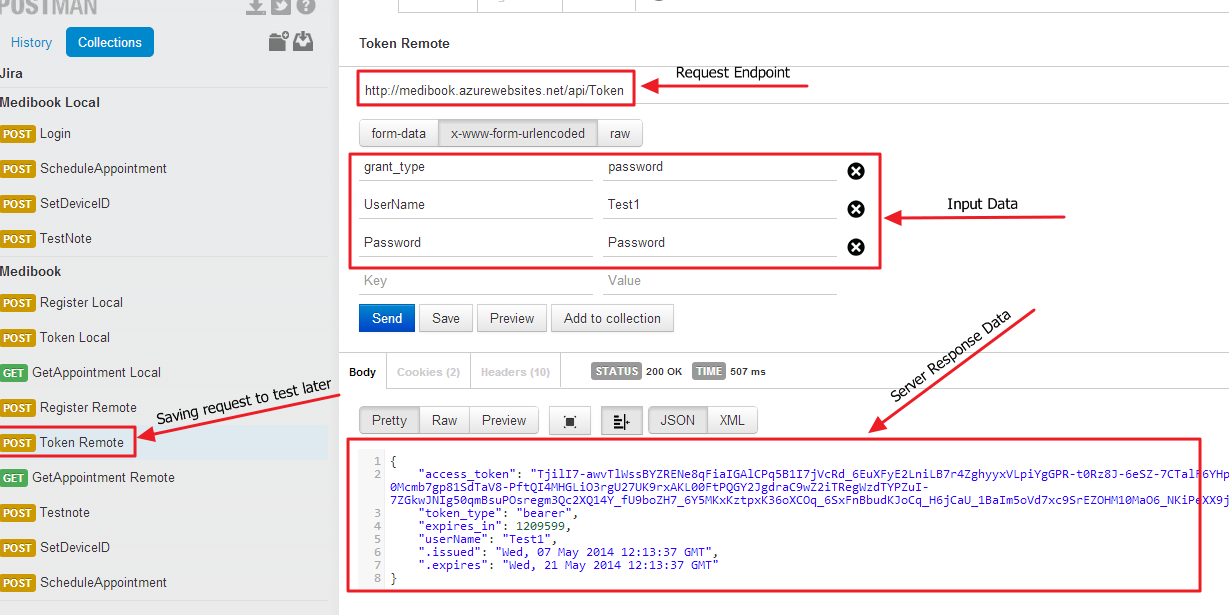
\includegraphics[width=\textwidth,height=\textheight,keepaspectratio]{Figures/Postman.png}
		\rule{35em}{0.5pt}
		\caption[Screenshot showing the use of Postman]{Screenshot showing the use of Postman}
	\label{fig:postman}
\end{figure}

\subsection{Organising Code}

A feature in most modern programming languages (including C\#) is the idea of modular design. This concept emphasises the separation of code functionality into interchangable modules. These modules can then reference other modules easily, and makes sharing code simpler.

Early on in the implementation stages, I found that I was having to duplicate some code and data values in both the client and the server application. This caused many unnecessary issues. For example, I would sometimes change one value and forget to change the other.

To solve this problem, I structured all of my code into separate modules so that they could easily be shared with both my client codebase and my server codebase. 

I organised the code into the following projects:

\begin{itemize}
	\item Medibook.Client.Android - The Android application that focuses entirely on Android specific design. \textit{References the Medibook.Client library.}
	\item Medibook.Client - The client library that contains all business logic that is shared with Android and IOS implementations. \textit{References the Medibook.Shared library.}
	\item Medibook.Server - The server application. \textit{References the Medibook.Shared library.}
	\item Medibook.Shared - The shared library that is shared between the Medibook.Client and Medibook.Server projects.
	\item Medibook.Testing - A unit-testing library that tests specific features of the client application and ensures they are working correctly.
\end{itemize}

With this modular setup, I was able to develop reusable code with no duplication, and allowing for a future iOS app to use the same business logic as the Android app.

With my projects setup, I began developing the basic infrastructure that that both the server application and android application would use.

\section{Server Structure}

Using the Asp.Net framework, the majority of the server's structure was already pre-ordained with a strong emphasis on using the Model-View-Controller design pattern. The server was therefore structured into two components:

\begin{itemize}
	\item Controllers - Containing the business logic and servicing all RESTful API request endpoints.
	\item Models - The data models for storing in the database and designing the structure of sent request data.
\end{itemize}

The server application did not have views because no interface was required for the prototype.

Most of the server implementation was done using controllers, as methods defined in a controller would become a web service endpoint which web-requests from the Android application could execute.

\begin{figure}[htbp]
	\centering
		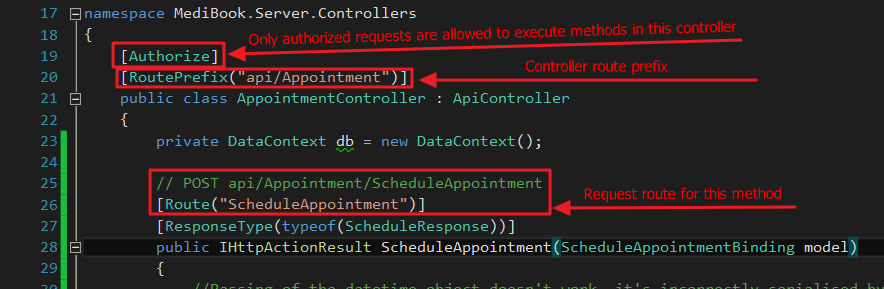
\includegraphics[width=\textwidth,height=\textheight,keepaspectratio]{Figures/ServerController.png}
		\rule{35em}{0.5pt}
		\caption[Example of a controller code showing authorised and routed requests]{Example of a controller code showing authorised and routed requests}
	\label{fig:servercontroller}
\end{figure}

Figure \ref{fig:servercontroller} shows the basic setup of an Asp.Net controller, including routing and authorisation. Every request method in this controller requires an authorised token.

\subsection{Authentication}

Authentication is supported by Asp.Net, so it's implementation was not as tricky as first thought in my original design.

By adding the [Authorize] attribute to a controller or individual request methods, Asp.Net recognises that this request (or all requests within the controller) requires authentication in order to access it.

To authorise requests, authorisation keys called 'Tokens' must be added to the requests authorisation header. If the authorisation header is missing or incorrect, the server will end the request and respond with the HTTP request code '401 Unauthorized'.

All requests sent to the server application require authentication, except the login and register requests, to ensure that patient data is kept secure.

\subsection{Routing}

When the server receives a request from the client, it will be in the form of a url. Asp.Net automatically parses this url into segments, in the form of '{controller}/{action}'.

After the segments have been parsed, it finds the correct controller defined with the controller segment, then the correct action method with the action segment and executes it, returning the output to the sender.

As a working example, if the client sent a request of 'Appointment/Schedule' would tell Asp.Net to look in the Appointment controller for the Schedule request method.

\subsection{Request Methods}

After the request has been routed to the correct method, the data needs to be de-serialised into a binding model.

This binding model defines the structure of the request, specifying the data types for each input parameter. It also provides validation tools to ensure that the data is input correctly.

\begin{figure}[htbp]
	\centering
		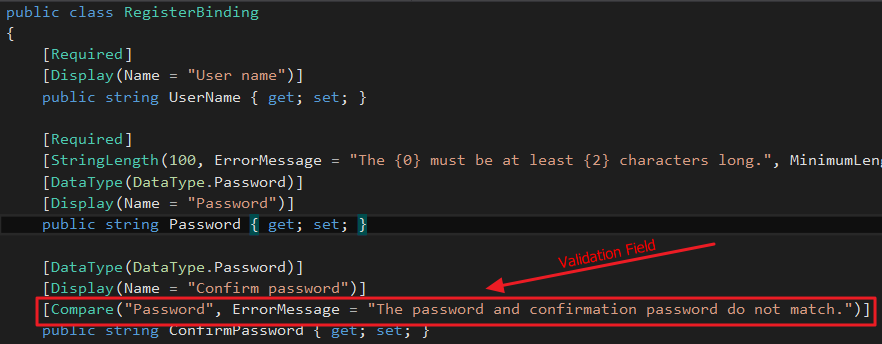
\includegraphics[width=\textwidth,height=\textheight,keepaspectratio]{Figures/bindingmodel.png}
		\rule{35em}{0.5pt}
		\caption[Example of a binding model associated with the register account request]{Example of a binding model associated with the register account request}
	\label{fig:bindingmodel}
\end{figure}

If the binding model is invalid for any reason, the server will end the request and respond with the HTTP status code '400 Bad request'. Error messages will also be returned if available, giving the request sender a reason as to why the request failed.

After the binding model is successfully validated, the request can be carried out the result is returned to the sender.

\subsection{Data Storage and Retrieval}

For data to be stored and retrieved easily, I used the Entity Framework library which integrates easily with ASP.Net and eliminates the need for most of the data access code. 

Two methods are available for database development when using Entity Framework; code first and database first. Code first allows you to let Entity Framework create and setup the database as you write your data models. Database first allows you to use entity framework to generate data models from an already existing database. For quick development, the code first method was chosen for this project.

\subsubsection{Data Models}

Data models work the same way as binding models, in that you design properties with data types for the data to bind to.

You can even use data models as binding models, which allowed me to reuse the same data models to serialise and de-serialise the data when sending to and from the client. I found however, that this was not always a good solution, as some data models have extra information that the client doesn't need (for example, the password property for a user model should not be sent to and from the client, especially when it is a different user).

Entity Framework data models also allow you to assign attributes to the properties such as '[key]' to modify it's behaviour as a primary key when stored in the database.

The best and most useful feature in entity framework is the automatic handling of foreign keys. If in one data model, you wish to reference a different data model, you can set the data type of that property to the data model's type and Entity Framework will do the rest of the hard work. This eliminates the need for any sql queries to fetch other data models that correspond to the foreign keys.

\begin{figure}[htbp]
	\centering
		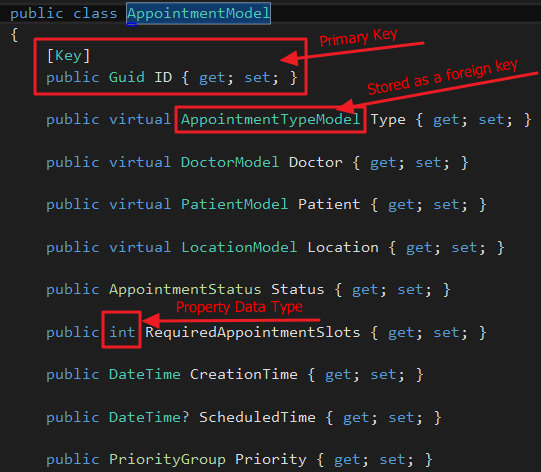
\includegraphics[width=\textwidth,height=\textheight,keepaspectratio]{Figures/EFModel.png}
		\rule{35em}{0.5pt}
		\caption[Example of an Entity Framework Data Model]{Example of an Entity Framework Data Model}
	\label{fig:efmodel}
\end{figure}

All data models were first designed by hand using entity relationship diagrams, however as the project progressed, these models became dramatically different as new features were added.

\begin{figure}[htbp]
	\centering
		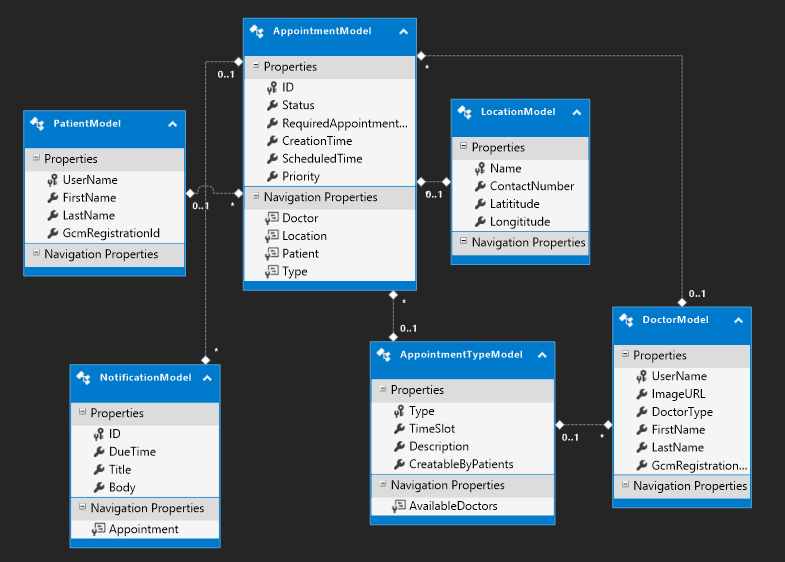
\includegraphics[width=\textwidth,height=\textheight,keepaspectratio]{Figures/database.png}
		\rule{35em}{0.5pt}
		\caption[The Final Entity Relationship Diagram]{The Final Entity Relationship Diagram}
	\label{fig:erdiagram}
\end{figure}

\subsubsection{Data Context}

When using Entity Framework, you must also create a data context.

This data context maps all of the entities and relationships that are defined in each data model to a database using the 'DbSet' class, allowing you to insert, update and delete data easily.

The data context also stores changes to the database transactionally, meaning that changes will only be written when calling the 'SaveChanges' method. This allows for changing the models with ease and not adding any performance issues as it writes unnecessary changes.

Using the data context, you can also query the data easily using LINQ.

\subsubsection{LINQ}

LINQ allows for the easy querying and updating data sets through C\# code. It follows an SQL-like syntax uses standard, easily learned patterns.

\begin{figure}[htbp]
	\centering
		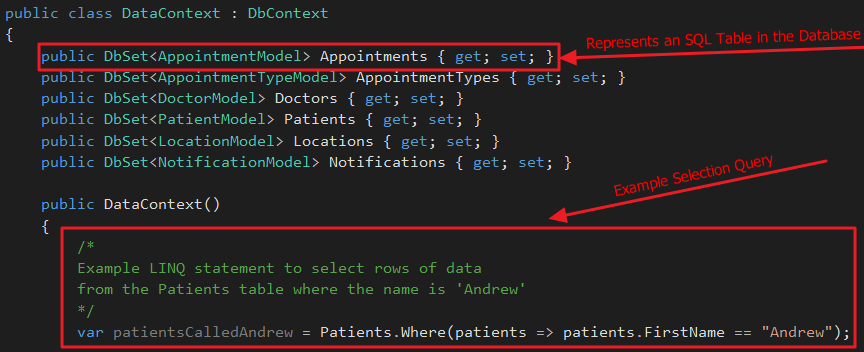
\includegraphics[width=\textwidth,height=\textheight,keepaspectratio]{Figures/EFContext.png}
		\rule{35em}{0.5pt}
		\caption[Example of the Entity Framework Data Context]{Example of the Entity Framework Data Context}
	\label{fig:efcontext}
\end{figure}

Using LINQ allowed me to select data easily through code, removing the need for direct SQL queries which could over complicate the process and introduce security vulnerabilities.

\subsubsection{Migrations}

After data models are created and added to the data context, Entity Framework allows you to migrate sample data when using the code first method. Migrations were therefore used to insert sample data into the database, such as appointments, patients, doctors, locations and any other information required for the prototype to function.

Besides adding data to a database, migrations also generate the SQL code necessary for making alterations to a database, using a version control system to allow different revisions of the database to be created. This allowed me to manage and update my remote database easily and not worry about adding new tables manually.

\section{Client Structure}

The client application is composed of two separate code bases, the client core library and the Android application.

\subsection{Client Core Library}

The client core uses the component based design pattern and is responsible for the majority of the applications business logic. This includes:

\begin{itemize}
	\item Sending and receiving requests from the server
	\item Storing data in the phone's memory and allowing multiple views to access it easily.
	\item Writing data to the phone's internal sqlite database
	\item Any other logic that isn't a platform specific feature
\end{itemize}

The client core is accessed via a static reference which means a component can be retrieved easily anywhere in the application. This turned out to be very useful for storing information that needed to be accessed by multiple parts of the client application.

\subsubsection{Creating Requests}

Besides storing data, the client core was also responsible for sending and receiving data from the server. To do this, the client needs to create a request and send it to the server so that it can receive data in return.

A client request is composed of three parts, the request url, the request parameters and the request method.

\begin{figure}[htbp]
	\centering
		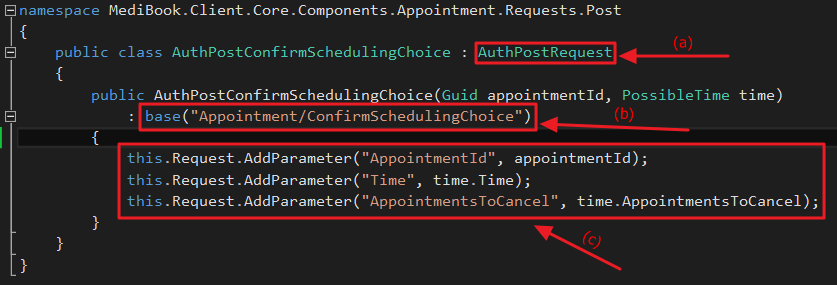
\includegraphics[width=\textwidth,height=\textheight,keepaspectratio]{Figures/ExampleRequest.png}
		\rule{35em}{0.5pt}
		\caption[Creation of a client request]{Creation of a client request}
	\label{fig:examplerequest}
\end{figure}

Figure \ref{fig:examplerequest} shows a request for confirming an appointment time with the server, specifying all three parts of the request.

Figure \ref{fig:examplerequest}(a) shows that this particular request extends the 'AuthPostRequest' which is retrieves the authorisation key from the account component and adds it to the request header. It also sets the request method to 'POST'.

Figure \ref{fig:examplerequest}(b) shows the request url, which it passes into the base constructor and is added to the request. This particular request targets the 'ConfirmSchedulingChoice' request method in the server's Appointment Controller.

Figure \ref{fig:examplerequest}(c) shows the parameters being added to the request. A parameter is a string key value pair which is added to the request so that it can be parsed by the server's request binding model.

\subsubsection{Request Response}

After the request has been created, the client executes it, sending it to the server and waiting for a response.

\begin{figure}[htbp]
	\centering
		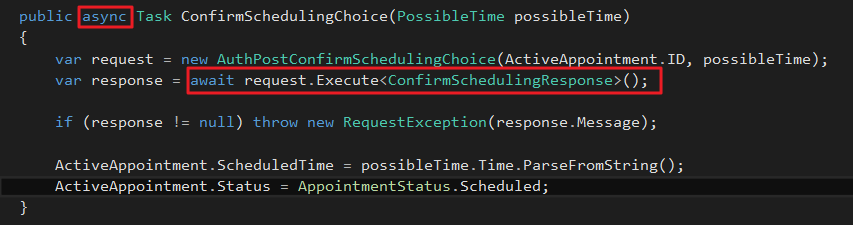
\includegraphics[width=\textwidth,height=\textheight,keepaspectratio]{Figures/ExampleResponse.png}
		\rule{35em}{0.5pt}
		\caption[Example of the client sending a request]{Example of the client sending a request}
	\label{fig:exampleresponse}
\end{figure}

In figure \ref{fig:exampleresponse}, you can see that the execution method also specifies a 'ConfirmSchedulingResponse' parameter. This is a binding model that the client then uses to de-serialise the response data into a usable form. This is similar to the server's implementation of the binding models and allows the specification of data types for the response data.

\subsubsection{Asynchronous Requests}

One problem I ran into when implementing requests was that my client application would halt until it received a response from the server (or the connection timed out). To solve this issue, I implemented asynchronous requests so that the program would continue functioning without waiting for a request to return its result first. This implementation uses the 'async await' feature in C\#. When the program hit's an await operator, the program will return to the request caller until a response is received. You can see this being used in figure \ref {fig:exampleresponse}.

This allowed me to effectively execute requests in the background without having an impact on the main application.

\subsection{Android Application}

The Android application, like the server application, uses the Model-View-Controller design pattern. The application structure was composed of a few base components; activities, intents, resources, layouts and services.

\subsubsection{Activities}

Android activities are the Android implementation of controllers. Usually tied to specific screens, they handle any logic required by the screen, including the creation of and switching to other activities if necessary.

Activities bind to an Android Layout and have several states that depend on if the activity is on the screen or not at the current time. For example, if the user presses the home button, the application is minimised and the activity is paused.

The Android client contained several activities, one for each screen available screen.

\subsubsection{Intents}

Android Intents are a description of a task to be performed. For example, when starting an activity, a 'StartActivity' intent must be created which takes the activity as a parameter. Intents are also useful for executing system tasks such as opening the phones dialer or calendar.

\subsubsection{Resources}

Android resources are all resources that the application uses, including pictures, layouts, sounds, constants and any other static data specific to the application.

As well as storing resources, the Android OS allows these resources to be easily accessed from within Activities.

The Android client uses resources to store all the layouts, fonts and images used in the application.

\subsubsection{Layouts}

Android layouts are views that define the visual structure for a user interface in the Android application.

Android provides an XML based API that corresponds to view classes and subclasses such as widgets that can be used in the user interface. It also allows you to attatch properties to these widgets that set it's position, id so the activity can find it, and many other variables that modify the widget's behaviour.

Xamarin also provides a drag and drop graphical user interface that allows for fast development of Android layouts for multiple devices.

\begin{sidewaysfigure}[htbp]
	\centering
		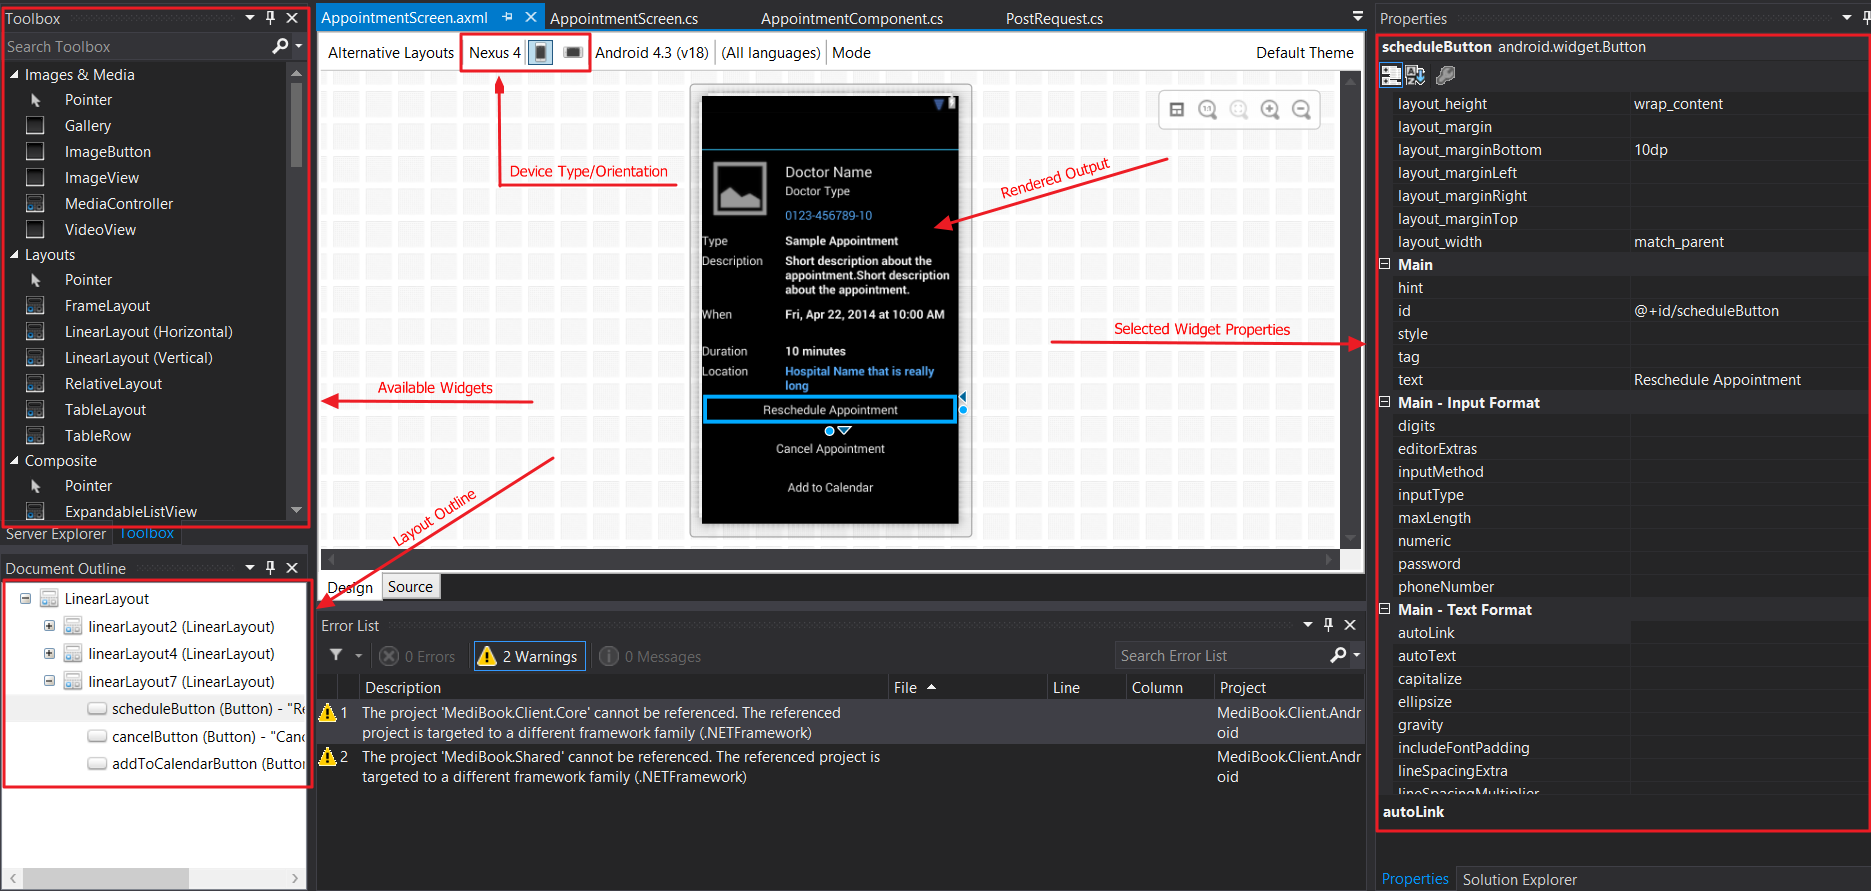
\includegraphics[width=\textwidth,height=\textheight,keepaspectratio]{Figures/XamarinLayoutDesigner.png}
		\rule{35em}{0.5pt}
		\caption[Screenshot showing the use of the Xamarin Layout Designer]{Screenshot showing the use of the Xamarin Layout Designer}
	\label{fig:layoutdesigner}
\end{sidewaysfigure}

As widgets are added to the design, the designer generates the XML source code for the layout. It also allows you to edit the layout code directly, re rendering any changes you make. This made it extremely useful as you did not need to compile and run the Android app (a process that can take a long time) every time you make a change to the design.

\subsubsection{Services}

Android services allow tasks to run in the background. They run in their own independent life cycle, meaning that they continue to function even when the app isn't running.

Android services were used to process incoming notifications sent from the google cloud messaging server. This allowed for the phone to receive messages whilst the app was not running and inform the user of changes to their appointments.

\section{Login and Authentication Feature}

With the basic infrastructure established, implementing the app authentication procedures was fairly simple.

To manage the authentication requests and logged in account, I created a component in the app core library which sends the login, registration and logout requests, as well as storing the current token used to sign authorised requests.

The Android visual implementation of this feature was also very straight forward. I created an activity and set it as the main launcher activity. This tells the Android OS to open this particular activity first when starting the app.

The login screen has two text input widgets that allows users to input their login details. Two buttons were also added which linked to the activity and sent the login and registration requests.

\subsection{Login Request}

The login request sends the user name and password input via the HTTPS protocol ensuring it is sent securely. If the login is successful, the server will respond with an access token, which is then stored in the account component.

\subsection{Registration Request}

When creating a new account, the following information is needed as parameters in the request:

\begin{itemize}
	\item UserName - unique user name required to log in with.
	\item Password - secret password required to log in with.
	\item AccountType - Either 'Patient' or 'Doctor'.
	\item FirstName
	\item LastName
\end{itemize}

Upon creating a new user account, the server will assign this account the role of either doctor or patient and add some example appointments to the account (for demonstration purposes). If the request is successful, the server responds the HTTP status code '200 OK'.

\subsection{Incorrect Input}

If either the login request or registration requests have incorrect input, the server will return the HTTP status code '401 Bad Request', also stating a reason as to why it failed such as 'Incorrect Password'. To give some feedback to the user, I needed to also implement an error text field in the layouts design which displayed when there was an error.

\subsection{Conclusion}

The login and authentication feature was surprisingly simple to implement due to the fact that Asp.Net has the majority of it built in. Combined with the role system, it made it very easy to identify users server side from the access token used to send the request, which became invaluable when deciding which appointments to send to the client.

I also found that because the login request was a perquisite for any further action of the app, I added a progress dialog widget which shows whilst the app is waiting for a response from the server. 

A dialog is a simple modal view, much like a pop up which displays data on top of the main layout. This simple visual feedback was effective at telling the user to be patient while the login request is in progress.

\section{Home Screen Feature}

For the home screen, two main features were required; the appointment list and the notification list. To allow for two separate lists on the same screen, the home screen was implemented as a tab activity.

\subsection{Tab Activity}

Tab activities allow easy navigation of two separate user interfaces and keep the design clear and separate. Navigation tabs are added to the top of the view in an action-bar to allow the user to easily switch between the different interfaces. 

To embed an interface into a tab, fragments must be created to host these interfaces. In this case, list fragments were used to display and manage the lists. The home screen layout then had a fragment container, which hosted the selected tab's corresponding fragment within it.

\subsection{Fragments}

Fragments are child activities that represent a portion of the user interface. Instead of embedding a layout into an activity, you can embed the layout into a fragment, and then add that fragment to an activity. This results in the ability to have multiple screens per activity.

\subsection{List Fragments}

By using the list fragment, I was able to create a layout design for a single item and assign it to an adapter.

Android adapters act as bridges between the layout and data for the view. This is required for a list fragment so that it knows how to bind the data to the layout correctly, allowing for dynamic lists to be created easily. It also adds functionality such as the order in which items appear in the list, as well as touch event handling to determine which item was selected.

By keeping a reference of the appointment/notification and it's index in the list, I was able to invoke a new activity with the relevant information needed when the user tapped on a list item.

\subsection{Retrieving Appointments}

Whilst implementing the client side, I used sample data to populate the data lists. Once the client implementation was complete, I started on implementing a request to fetch all of the appointments that are assigned to a patient.

\subsubsection{Server Side Request}

I started by creating a new controller in my server project to manage appointment requests, setting all requests in the controller to require authentication.

This allowed me to not only keep the information secure, but also fetch the patient's identity easily by using the Asp.Net property 'User.Identity' that is available in all authorised requests. The Asp.Net populates this by checking the used token against logged in sessions, retrieving the correct identity from the session.

\subsubsection{Appointment Model}

An appointment model was created based on my original ER Diagram and put in the shared project so that both the client and server could access it. This was to allow the server to store, retrieve and send the data to the client, as well as allowing the client to use the model to de-serialise the returned data from the request. 

The model was then added to the data context and a new reference of the data context was created within the appointment controller.

With the patient's user name available, it was very easy therefore to retrieve all appointments linked with that user name, returning them in the request.

Figure \ref{fig:efmodel} shows the appointment model and it's properties. Although not all of the information was relevant for the list, this query sent of the entire appointment model so that it could later be used in the Appointment Information Screen, removing the need for a second query to be executed.

\subsection{Action Bar}

With the relevant appointments being successfully retrieved from the server, the appointments were stored in the appointment component and injected into the list adapter.

Later on in the implementation, I found that these appointments were becoming out of date. I found that a good solution to this was to create a button to manually fetch appointments from the server and repopulate the list.

The list view took up the entire screen and I did not want to remove focus from it as it was the main feature, so I created a second action bar above the tab bar.

To implement this, I utilised the 'App Compat' Android library which adds a top bar menu to all your activities. This made it very simple to add button tabs at the top of your screen, as well as displaying the name of the current screen to make navigation of the app easier.

A refresh button was added which, when pressed, would request the appointment data from the server again. A rotating progress icon was also added to the button to show whilst the request was in progress. Another solution to ensure appointments were kept up to date was the adding of the request to the 'OnActivityResumed' method, which executes whenever the activity becomes visible again. This resulted in the app refreshing the appointments whenever the home screen was re-opened.

A logout button was also added to the bar to allow the switching of accounts and returned the user to the login screen.

\section{Appointment Information Feature}

With the appointments already retrieved, implementing the appointment information feature was simple. When a appointment was tapped on the list, it would set the 'CurrentAppointmentOpen' property to the relevant appointment in the appointment component. It then opened a new activity for the information screen.

To create the information screen, I used the layout designer to create a layout with the required widgets.

When the appointment information activity was started, it displayed the layout and retrieved the relevant appointment from the appointment component. It then assigned the text fields in the layout to the relevant information in appointment so that the information was specific to the requested appointment.

\subsection{Doctor's Image}

One technical challenge faced was providing the doctor's image for this feature. Images are normally added to the resources folder, however this would not be an effective solution because the app would then need to be updated whenever a new doctor is added.

Due to having a limitation on requests were only textual information could be sent, I added an image url to the doctor model. This url pointed to a web server hosting the image where by using a separate request, it could be retrieved.

Upon opening the activity, the image widget therefore contains a place holder image while it downloads the actual image onto the phone from the external server. This worked effectively and allowed doctor's portrait images to be changed remotely on the server without having to update the app.

\subsection{Buttons}

Several buttons were also created to allow the patient to easily schedule, re-schedule and cancel their appointments.

Upon pressing these buttons, the layout would invoke a method in the activity that carried out the functionality. The schedule button would create a new activity that took the user to the scheduling screen. The cancel button would send a cancel appointment request, sending the appointment id to the server in the request.

\subsection{Action Bar}

An action bar was also added to the appointment information screen using the same method as in the home screen. In the action bar, a map button was added that created a new activity for the map view, as well as a back button that finished the current activity and returned to the home screen.

\subsection{Dialer}

By tapping the contact number text field, the activity was required to open the phones dialer with the same number.

This was relatively simple to implement. The text field's 'OnClick' property was utilised to invoke an 'OpenDialer' method in the activity. This method created an Android Intent that told the Android OS to open the dialer action of the phone. The 'SetData' field to set the number from the appointment so that the dialer had access to the relevant information

One issue I had was that in order for the dialer to parse the number correctly, the string value passed to it must be prefixed with 'tel:', which was missed in the first iteration of it's implementation.

\section{Calendar Feature}

The calendar feature added a button to the appointment information screen, allowing the user to add (or remove) the appointment details to their phone calendar.

Accessing the phone calendar was a complex process, requiring Android app permissions, content resolvers to retrieve the information and extensive reading of poor Android documentation.

\subsection{Calendar Querying}

Android is a privilege-separated operating system, requiring all applications to request privilege permissions in the applications manifest. Certain restricted features are not available until these privileges have been added, which prompts the user upon the install of the application of the restricted features it has access to.

The app manifest is essentially the Android application's configuration file, specifying which android sdk version it uses and any permissions it requires. The calendar access required the permissions 'READ\_CALENDAR' and 'WRITE\_CALENDAR', prompting the user that the application was able to read and write from the calendar.

Content resolvers are used to manage access to a structured set of data in Android. One problem that content resolvers solve is data access conflicts, when multiple Android applications are modifying the same data at the same time.

As an added feature, I wanted to query the the calendar to see if the appointment was already added. This would allow me to swap the 'Add to Calendar' button with a 'Remove from Calendar' button.

To do this, I needed to create a content resolver to fetch the correct calendar id, and then create a second content resolver to check if any entries existed in that calendar.

\subsection{Issues}

This feature started out relatively simple, but became increasingly problematic because Android has lots of deprecated methods of accessing calendar information. Deprecated methods are old ways implementing a feature, but are left in the Android sdk to preserve backwards compatibility.

One issue I encountered was that upon removing an appointment from the calendar, I found that it still existed when I queried it. After reading different versions of the same Android documentation, I found the most up to date implementation and discovered that when removing an entry from the calendar, the latest version of Android sets a 'removed' field boolean to true rather than deleting the entry. Although this was very simple to fix (by checking this 'removed' field), it took me many hours to find out why my entries were not being deleted.

Another issue I encountered was that upon cancelling an appointment, it was not removed from the calendar, resulting in it displaying an incorrect time. This was fixed by calling the 'RemoveFromCalendar' method when an appointment time is updated.

\section{Location and Map Feature}

The location and map feature aimed to prevent patients getting lost on their way to the appointment. By tapping on the location name or selecting the map button in the action bar of the appointment information screen, the app opened the map activity.

The map activity was very simple to implement. Android has a 'MapFragment' class designed for embedding 'Google Maps' directly into apps, providing a dynamic map and useful helper methods to manipulate it. 

\subsection{Google Maps API}

To utilise the map fragment, Google requests that you provide your application API key in the app's manifest file. To obtain a key, you must register your app with google through the google developer portal, a process that takes just a few minutes, is free of charge and allows you to access many useful API's.

After adding the API key provided, the map fragment was able to render a map within the app.

\subsection{Placing a marker}

After implementing the app map, the solution required a marker on the map displaying the location position and name. This required me to change the location data model, adding latitude and longitude properties to it so that the server could send the correct location.

Once the marker was set on the map, the map's settings were changed so that the map view would open with the marker centred.

\section{Appointment Scheduling Feature}

The main feature of the application was the ability to schedule and reschedule appointments. This was the hardest feature of the project aside from the initial design. This was primarily down to the complexity of the scheduling process, resulting in many obstacles that needed to be avoided. To begin implementing feature, I created several workflow diagrams to emulate the scheduling of an appointment by hand. Different scenarios were drafted, providing a set of clear instructions that the server and client carried out for each one. By modeling out the scheduling process by hand, it made the implementation much easier.

\subsection{Date Picker}

To start scheduling an appointment, a button was added to the appointment information screen that invoked a schedule appointment activity. This activity had three buttons in it's layout; a time picker button, a confirmation button and a cancel button.

When selecting the time picker, a dialog was created that showed a date and time slider. Care was taken to ensure that the user could not pick a time before the current date. After the user had inputed a time and date, the confirmation button would execute the request.

\subsection{Example Scheduler}

To emulate a real world scheduling algorithm, I implemented an 'Example Scheduler' program to find an appointment for the user. The aim of this program was to return an appointment time as close to the requested time as possible. The first obstacle to overcome was appointment conflicts.

To detect conflicts, the scheduler queries the appointment database for all appointments where the times overlap. It first calculates the time range of the requested time using the appointment duration. If any scheduled appointments overlap, the scheduler will flag the time as conflicting. 

The scheduler deals with conflicts in two ways; using a priority based system to cancel other appointments or suggesting other available times. Every appointment is assigned a priority in the appointment model, based on how vital it is that this appointment is scheduled soon. This is used to compare how important appointments are relative to each other and whether an appointment can be rearranged or not.

If the conflicting appointments are less important than the requested appointment, the scheduler will cancel them and inform the patients and doctors by sending notifications to the devices. If the priorities are the same or the requested appointment is less important, the scheduler will find three possible times as close as possible to the requested time. It does this by incrementing the requested time hourly and repeating the conflict detection process again until it finds three possible appointments.

\subsection{Confirming the Appointment}

If the scheduler returns one result, the server will confirm the appointment and respond to the client that the appointment has been scheduled. Otherwise, it will return the three possible choices.

If three choices are received from the server by the client, the activity will start a new scheduling choice activity screen, which displays the times to the patient and asks them to choose one. Upon choosing a time, the client will send a confirmation request to the server to schedule the appointment.

\subsection{Time issue}

One issue I ran into when implementing this were time zones. The time calculated on the phone was in the time-zone 'British Summer Time (BST)', which was an hour ahead of the time calculated on the server 'Coordinated Universal Time (UTC)'. This caused many problems when sending and receiving times because they would become out of sync. 

My first attempt to solve this was simple, change the time zone that the server is running on. I later found that this was not possible because the server was hosted on the Windows Azure Cloud, designed to be run in any geographical location and therefore prohibiting any changing of the time-zone. The app had to be therefore designed to run in any time zone.

The second attempt to solve this utilised C\#'s 'TimeZoneInfo' class which allows for the conversion of times to different timezones. I later found that due to the nature of the the Monodroid compiler that allowed C\# to be transformed into Java based code, no regional information was available and the 'TimeZoneInfo' class was unable to function correctly.

I did not find a solution to this besides manually offsetting the between UTC and UTC + 1 when times are sent and received. This will not work forever, as when the phone's time zone changes from 'British Summer Time' back to 'Greenwich Mean Time (GMT)' the offset will still be in effect. However, as this was a prototype, this bug was not a priority.

\section{Notification Feature}

The last feature of the application implemented push notifications. The need for notifications was important for reminding patients about their appointments and providing live communication with them. Push notifications utilised the Google Cloud Messaging API to send the message and Android Services to process the messages as they are received.

Google Cloud Messaging was chosen to provide push notifications due to it's simplicity to implement, as well as being optimised for battery efficiency and poor bandwidth.

\subsection{GCM Service}

In order for the Android device to receive GCM messages, it must start a service that runs as a background process on the device. This service registers the application with the GCM Service that runs natively on all Android devices. Upon registration, a device registration id is provided which is used to determine which device to send the message payload to. This registration id must therefore be sent to the server and stored in the patients data model so that the server can successfully send messages to the correct device.

Besides device registration, the background service is also responsible for handling messages that are received from the GCM Server. Upon receiving a message, the 'OnMessage' method is triggered in the service with the resulting payload. This method adds the notification to the notification list in the home screen and shows creates a local notification to inform the user that they have a new message.

\subsection{Sending of GCM messages}

In order to create a GCM message, a rest request must be sent to the GCM servers. The request must contain the Android application's API key, the registration id of the patient's device and the message payload.

The API key is retrieved the same way as the Google Maps API key was retrieved, through the Google Developer Portal. This informs the GCM Service on the Android device which application the message is related to.

The registration id is sent via a web request from the Android app and the Account Component assigns this id to the relevant patient model. This means that no notifications can be sent to the device until it has retrieved this request from the Android client.

The message payload contains any data that is sent to the device, such as the notification message and the relevant appointment id. Different types of notifications are therefore created easily by specifying custom data in the payload.

\subsection{Observer}

Another important feature of sending notifications was the scheduling of them. Notifications need to be sent at specific times to remind patients about various aspects of the appointment. To do this, an Observer service was implemented on the Asp.Net server that runs in the background. This utilises the Timer method in the Observable class to execute notifications at a set time.

This allows for reminder notifications to be queued easily as an appointment is scheduled. The prototype automatically schedules a notification to be sent an hour prior to an appointment's start time.

%---------------------------------------------------------------------------------------- 
% Chapter Template

\chapter{Testing and Evaluation} % Main chapter title

\label{Chapter6} % Change X to a consecutive number; for referencing this chapter elsewhere, use \ref{ChapterX}

\lhead{Chapter 6. \emph{Testing and Evaluation}} % Change X to a consecutive number; this is for the header on each page - perhaps a shortened title

%----------------------------------------------------------------------------------------
\section{Introduction}

This chapter will focus on the testing and evaluation of the solution implemented. In order to evaluate how suitable the solution is at fulfilling the requirements, user based assessments were performed to collect feedback.

\section{Testing}

Before the assessments could begin, the application needed to be tested thoroughly so that the it would perform correctly and the feedback from the assessments would be most valuable. The testing was split into two sections, unit testing and functional testing.

\subsection{Unit Testing}

Unit testing is a form of automated software testing that individual executes portions of the code and validates whether the output is desirable or not. Unit testing is very useful in iterative based development where testing needs to be repeated often to ensure older features do not get broken by newer ones. This is a common issue in software programming, especially when many developers are working on the same code base and don't fully understand the entirety of it, resulting in undesirable changes and side effects commonly occurring.

Although some unit tests were written for this project using the 'Visual Studio Unit Testing Framework', I decided that the time cost for implementing the tests was not worth the output, especially as the project had a fairly small code base and I was the sole developer. Most of the features were also created independently of each other, resulting in a smaller risk of them modifying each others functionality.

\subsection{Functional Testing}

Functional testing is a requirement in any software development project to ensure it is ready for release. Functional testing is the manual act of testing the functionality of an application, just like an end user would. This helps to  identify functions of the application that are broken or poorly designed, ensuring that these functions do not make it to the end user.

\subsubsection{Testing Methodology}

In order to test the app's functions, an initial regression test was used. Regression testing is a form of functional software testing that seeks to uncover software bugs within certain features of a software application. An initial regression test includes all features implemented in the prototype. As extra features are added at a later date, new regression tests must be made for these features. Only once all features are tested and pass can the application be signed off for release.

To start regression testing, an extensive list of all the app's features was made. This test list comprised of the following information:

\begin{itemize}
	\item Test Number - A unique number for easily identifying the test.
	\item Feature Category - The category that the feature belongs to.
	\item Feature Type - The type of feature it is.
	\item Action - A description of feature and its desired effect.
	\item Pass/Fail - Whether the test was successful or not.
	\item Comments - Reason as to why the test failed or any improvements that could be made.
\end{itemize}

With the test list formulated, each feature was tested multiple times to determine if they should pass or fail by comparing the test action to the actual result.

\subsubsection{Results}

\begin{figure}[htbp]
	\centering
		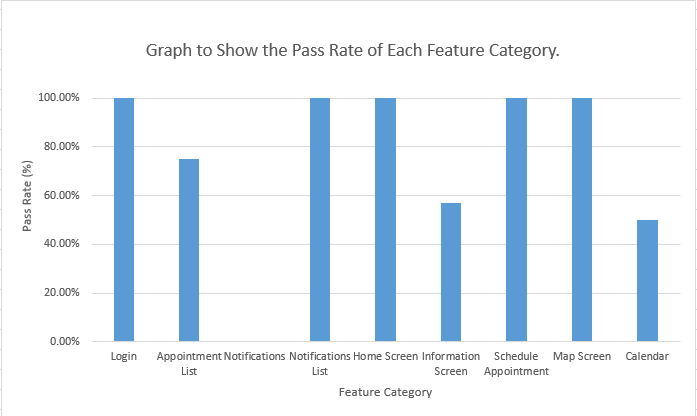
\includegraphics[width=\textwidth,height=\textheight,keepaspectratio]{Figures/FunctionalTestResults.png}
		\rule{35em}{0.5pt}
		\caption[Graph to show the pass rate of each feature category.]{Graph to show the pass rate of each feature category.}
	\label{fig:functionaltestresults}
\end{figure}

Appendix C shows the results of the initial regression test. The initial results showed that although the majority of the app was working as intended, the notification feature category was completely broken and needed fixed prior to the user based assessments.

\subsection{Further Testing}

Although aspects of the mobile application were fully tested, most of the testing was focused on the user interface and testing of the server was ignored. Further testing must be done to analyse how the system would perform in a production environment. Due the the system being a prototype, it was not necessary for this project.

\subsubsection{Load testing}

In order to assess how many concurrent users can successfully use the system before issues occur, load testing must be performed. This is a process where test accounts are created and accessed at the same time, which is repeated until performance  or other issues begin to occur. This helps to prepare for user demand and outline efficiency issues or the hardware requirements for the system prior to it being launched.

\subsubsection{Concurrency Issues}

One hypothetical issue came to mind when implementing the prototype; what happens when two separate users schedule the same appointment at the same time. Although the system is designed to be flexible enough such that these issues would not have a fatal effect on the system, it would likely create an error that is not currently handled by the client application. Many issues like this could exist, and features would have to be tested thoroughly to discover them all.

\subsection{Conclusion}

With the test results collected, any failures were investigated and the specific action was re-implemented. Final regression tests were repeated until all failures were passed and the prototype was ready for evaluation.

Further performance testing and analysis of the applications resource usage could also have been performed, but slow/poor performance was not picked up by the functional testing and was therefore deemed unnecessary.

%----------------------------------------------------------------------------------------

\section{Evaluation}

After testing was completed and the app was in a stable state, the evaluation could commence.

As stated in Section 2.5, I wanted to evaluate the solution based on the following questions:

\begin{itemize}
	\item How easy to use is the mobile application?
	\item Does the solution work? Does it fail occasionally?
	\item Is the solution missing key features?
	\item Would patients find the mobile application useful?
	\item Does the solution reduce wasted appointments?
	\item Does the solution reduce staff resources required for managing appointments?
	\item Does the solution increase the user experience when managing appointments?
\end{itemize}

In order to evaluate these questions, three methods of evaluation were proposed, user observation, user feedback and trials in real hospital environments.

\subsection{Evaluation of Methodology}

Whilst designing and implementing the prototype, it became apparent that the proposed solution was not ideal. Firstly, the solution could wrongly encourage patients to reschedule appointments when it is unnecessary. This would, without a doubt put strain on the system, making it hard for medical staff to constantly adapt to changes in the schedule.

This is however a hypothetical problem. When patients are faced with the probable long waiting times that they would in an hospital environment, it would be undesirable for them to reschedule appointments often. Trials of the proposed system would have to be run to determine whether the additional strain would exist or not.

Another problem the solution faces is that it would not be able to replace the current system entirely, as not all patients have access to smart devices and internet access. The system would have to be integrated alongside other systems in place, which could prove challenging with clinics that still use paper based approaches or rely on staff members for appointment management. As the number of patients without internet access is a growing minority, this may not be as problematic as first thought. Also, as the solution is designed to be platform independent, web interfaces could be set up in clinics and hospitals to accommodate for this, or even dedicated staff members to manage appointments through the system on a patient's behalf.

\subsection{Controlled Trials}

In order to evaluate the effects of the solution on staff resources and appointment wastage, trials would need to be carried out in real clinics and hospitals. This would produce statistical data that could then be compared with a control group who use the standard methods of appointment scheduling available today.

Unfortunately, it was not possible to conduct clinical trials for this project due to insufficient resources and the time restrictions involved. Despite this, I was able to conduct the user evaluation successfully and collected good feedback to evaluate the user experience of the application.

\subsection{User Observation}

User observation was carried out on a ten willing participants who were given a sheet with a list of tasks that they had to attempt (see Appendix E). Tasks were deliberately designed to be vague, not offering any instructions on how to complete a task. By designing the tasks this way, it demonstrated the applications usability and aimed to identify areas that were not intuitive.

Applicants were also provided with a test account with three hypothetical appointments already set up. The first two appointments were unscheduled to demonstrate the scheduling functionality of the app, and the third demonstrated the synchronisation with the phones calendar feature.

From observing the entire applicant group, none had issues completing all of the tasks given. Feedback was generally very positive for most of the features except the scheduling process. Some applicants showed signs of annoyance when trying to get the desired appointment which required a trial and error approach of inputting times and seeing if they were taken. Although the system offered a selection of choices close to the input time, this was not desirable for a user with a specific set of dates and times that they were available on.

Applicants also queried for a way to manage notifications, turning certain notifications on and off and highlighting a useful extension that could be added in the future.

\subsection{User Questionnaire}

The user questionnaire was designed (see Appendix F) to collect useful feedback and carried out after the user observation on the same participant group. The questionnaire consisted of numerical ratings of the mobile application and the following graph was composed from the average ratings provided from all ten applicants:

\begin{figure}[htbp]
	\centering
		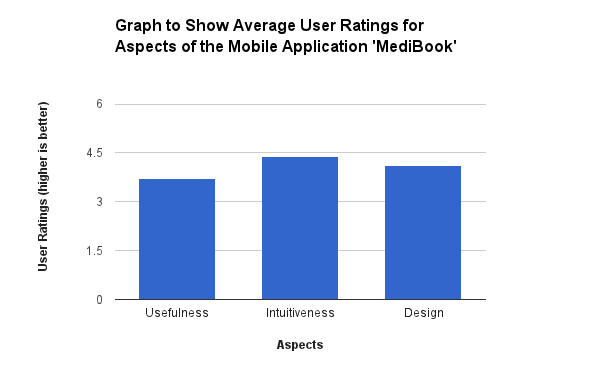
\includegraphics[width=\textwidth,height=\textheight,keepaspectratio]{Figures/AverageRatings.png}
		\rule{35em}{0.5pt}
		\caption[Graph to Show the Average User Ratings Collected from the User Questionnaire]{Graph to Show the Average User Ratings Collected from the User Questionnaire}
	\label{fig:questionnaireresults}
\end{figure}

The questionnaire also provided ways for the applicants to give feedback and suggestions. Some useful feedback included the suggestion of disabling unavailable times from the app's time picker fix the trial and error approach currently implemented. Some users also suggested possible future extensions such as using the notification feature for scheduling a patients medication, also providing them with prescription information and pharmacies located near the patient.

\subsection{Further Evaluation}

Besides the methods discussed above, many aspects are missing from the evaluation due to time restrictions and further evaluation could be performed in the future.

\subsubsection{Training}

Although the user evaluation showed that the app was intuitive, all participants admitted to owning their own smart device and had general knowledge on how to operate an Android application.

Further testing could be performed on a test group consisting of people who are not technically proficient. This would give a better analysis on training requirements and would help outline documentation and a manual for the applications operation.

\subsubsection{Comparison with Phone Appointment Booking}

As identified in the problem description, one of the main methods for booking a medical appointment currently is over the telephone, so further evaluation could be performed to identify the strengths and shortcomings of the prototype when compared with a telephone booking.

Participants would be asked to first book an appointment over the telephone, and then book the same appointment through the mobile application. They would then be interviewed on their findings. Some useful questions could be asked to compare the mobile app with telephone appointment bookings:

\begin{itemize}
	\item Is it faster to book via mobile?
	\item How many telephone staff members were required to fulfil demand?
	\item How many staff members were required to maintain the mobile application?
	\item Was more information available by telephone?
\end{itemize}

\subsection{conclusion}

Based on the findings obtained by the user evaluation, the prototype application can be judged as a success in terms of providing a good user experience. It is easy to use, did not fail during the user evaluation and participants found that it was useful. Although it was missing some features such as disabling unavailable times from the time picker, these could be implemented easily in the future.

However, although the user evaluation was successful, many other observations required for the evaluation of this system depend upon real world scenarios. More testing and evaluation of the system being used in real hospital and clinic environments would have to be executed before it could be deemed a success.

%---------------------------------------------------------------------------------------- 
% Chapter Template

\chapter{Project Conclusion} % Main chapter title

\label{Chapter7} % Change X to a consecutive number; for referencing this chapter elsewhere, use \ref{ChapterX}

\lhead{Chapter 7. \emph{Project Conclusion}} % Change X to a consecutive number; this is for the header on each page - perhaps a shortened title

%----------------------------------------------------------------------------------------
To be written

\section{Objectives}
\section{Further Extensions}
\section{Future Extensions}
\section{Final Conclusion}

%---------------------------------------------------------------------------------------- 

%----------------------------------------------------------------------------------------
%	THESIS CONTENT - APPENDICES
%----------------------------------------------------------------------------------------

\addtocontents{toc}{\vspace{2em}} % Add a gap in the Contents, for aesthetics

\appendix % Cue to tell LaTeX that the following 'chapters' are Appendices

% Include the appendices of the thesis as separate files from the Appendices folder
% Uncomment the lines as you write the Appendices

% Appendix Template

\chapter{Personal Reflection} % Main appendix title

\label{AppendixA} % Change X to a consecutive letter; for referencing this appendix elsewhere, use \ref{AppendixX}

\lhead{Appendix A. \emph{Personal Reflection}} % Change X to a consecutive letter; this is for the header on each page - perhaps a shortened title

%talk about why you chose the project, 
When first faced with my final year project, I was overwhelmed with choice. Throughout my university career, I have rarely had the freedom to choose precisely what I wanted to learn. It is therefore very tempting to pick an area that you already know well, with very little learning benefit.

To overcome this, I set out a list of personal goals that I wanted to achieve by doing a project, which helped me narrow my choices:

\begin{itemize}
	\item I wanted to learn how to build mobile applications.
	\item I wanted to learn how to build an adaptable, scalable server.
	\item I wanted to provide a tool that would potentially help people.
\end{itemize}

It became clear after reading through project choices submitted by lecturers that none of them would help me obtain my goals. Thankfully, with the help of my supervisor, I was able to draft out a suitable project that was suitable enough to achieve both the universities and my own goals.

%talk about project planning, lack of deadlines
The second challenge I faced was project planning. I was not used to the lack of deadlines, and it took a long time for me to get started on my project. I overcame this problem through the use of personal deadlines. Although creating a Gantt chart helped keep track of the project's progress, I did not keep to it initially. I discovered the hard way by falling behind, and I spent many painful hours catching up to my initial schedule.

Another issue I faced with the project planning was encountering entire tasks. Although I had split my project into sub tasks such as implementation, it seemed very daunting when first facing them. To overcome this, I used project management tools like 'Trello' to split tasks down into subtasks, leave comments that I could remember and plan features out. This helped overcome the initial stress involved when planning specific parts of the project, making todo lists and remembering issues that occured for when you write the report. I found this far more valuable than keeping a journal as the user interface is very flexible and appealing.

The aspect of the project I enjoyed the most was the implementation. Although I had outlined things that I wanted to learn by doing this project, I learned far more during implementation due to issues that I had not even considered. An example of this was my problems with time synchronisation across multiple regions around the world, requiring me to look into solutions to this and learning about the various practices involved in geographical programming.

Besides implementation, this project has taught me invaluable skills that I will no doubt be utilising for years to come. I learnt how to formulate a report, conduct evaluation on research literature, software testing, communicating with various entities to get project resources, user based evaluation and many more skills involved.

Ultimately, my final year project was the highlight of my degree for me. It has been the greatest learning opportunity and challenge that I have faced in my university career, and I am grateful for having the opportunity to participate in it.

Finally, I will summarise my findings to compose this list of recommendations for future students:

\begin{itemize}
	\item Don't pick a project that sounds easy, choose what \bf{you} want to learn first, then find a project that fits your learning goals.
	\item Make personal deadlines to achieve project tasks on time. Plan accordingly in advance!
	\item Use tools such as Trello to plan your implementation, write down any issues you encounter so that you can discuss them in your report.
	\item Plan your evaluation in advance, make sure you've finished your implementation with plenty time to spare!
	\item Backup your project in multiple places, Github and dropbox are great tools!
	\item Enjoy your project and make it what you want it to be.
	\item Give yourself extra time to deal with unforeseen errors, they are a certainty.
\end{itemize}

% Appendix Template

\chapter{External Resources and Materials} % Main appendix title

\label{AppendixB} % Change X to a consecutive letter; for referencing this appendix elsewhere, use \ref{AppendixX}

\lhead{Appendix B. \emph{External Resources and Materials}} % Change X to a consecutive letter; this is for the header on each page - perhaps a shortened title

\begin{itemize}
	\item Use of the Xamarin Framework to develop the Android application obtainable at:\\ \url{http://xamarin.com/}
	\item Use of the ASP.Net Framework to develop the Server application obtainable at:\\ \url{http://asp.net}
	\item Use of the Entity Framework library to crate and manage SQL databases in C\#, available at: \url{http://msdn.microsoft.com/en-gb/data/ef.aspx}
	\item Use of the Rest Sharp library for the creation of RESTful web requests and the de-serialisation of response data, available at: \url{https://github.com/restsharp/RestSharp}
	\item Use of the GCM Client library for integrating GCM with Xamarin, obtainable at:\\ \url{https://github.com/Redth/GCM.Client}
	\item Windows Azure was used to host the server application and the database, available at:
	\url{http://medibook.azurewebsites.net/}
	\item Use of the Masters/Doctoral Thesis Latex Template for the creation of this report, obtainable at: \url{http://www.latextemplates.com/template/masters-doctoral-thesis}
\end{itemize}
% Appendix Template

\chapter{How ethical issues are addressed} % Main appendix title

\label{AppendixA} % Change X to a consecutive letter; for referencing this appendix elsewhere, use \ref{AppendixX}

\lhead{Appendix A. \emph{How ethical issues are addressed}} % Change X to a consecutive letter; this is for the header on each page - perhaps a shortened title

\section{Introduction}

This section describes the ethical issues involved throughout the project. I also propose techniques for solving and minimising these issues.

\section{Project background}

A few ethical issues arise from the projects aims and objectives. Firstly, personal data will be used and stored in order to optimise the projects aims. Secondly, the project aims to optimise the scheduling process, which could make some employees jobs redundant.

\subsection{Personal Data}

Personal data will be stored and used both locally (on the mobile device) and on an external server to try and optimise scheduling software. It may also be required to transmit this data regularly to keep the system running effectively.

This brings into security issues, as the data could be very valuable to certain individuals for marketing or other purposes. In order to solve this, several areas should considered:

\begin{itemize}
	\item Patients must be informed about what data is being stored and why
	\item The system should be as secure as possible with the current technology
	\item The data should be as anonymous as possible, with no individual besides its owner having access to it.
\end{itemize}

\subsection{Employee Downsizing}

The system aims to optimise the scheduling process and would replace a lot of the manual labour involved. It is therefore possible that the system would make some employees redundant.

Although this system aims to optimise the current system, it would not be able to replace it entirely, and so not all jobs would be lost. Also, this is only a short term problem, and with more training, employees could be allocated elsewhere.

\section{Testing and Evaluation}

In order to evaluate this project, I plan to perform user based assessments.

\subsection{User Based Assessments}

When performing user based assessments, care must be taken to ensure that participants are well informed of their rights, what the project is about and how their feedback would be stored and used. The participants data would also need to be stored anonymously to preserve confidentiality.

To ensure this is done correctly, the following steps will be taken:

\begin{enumerate}
	\item The nature of the project will be explained to the user.
	\item The user will be informed that their opinions will be used and stored both anonymously and securely.
	\item The user will be informed that they can stop the assessment at any time
	\item The user will be asked to sign a consent form to confirm that they have agreed to take part and that their data can be used to evaluate the project
	\item The data will be collected and stored anonymously
\end{enumerate}
% Appendix Template

\chapter{Regression Test} % Main appendix title

\label{AppendixD} % Change X to a consecutive letter; for referencing this appendix elsewhere, use \ref{AppendixX}

\lhead{Appendix D. \emph{Regression Test}} % Change X to a consecutive letter; this is for the header on each page - perhaps a shortened title

\begin{table}[h]
\centering
\resizebox{\textwidth}{!}{%
\begin{tabular}{|m{1cm}|m{3cm}|m{4cm}|m{6cm}|m{2cm}|m{6cm}|}
\hline
Test \# & Feature Category              & Feature Type                 & Action                                                                                                                    & Pass / Fail & Comments / Fault Description                                                                                                                               \\ \hline
1       & Login                         & Login Button                 & Logs the user in and progresses to the appointment list screen                                                            & Pass        &                                                                                                                                                            \\ \hline
2       & Login                         & Register Button              & Registers the user using the entered username and password, logs the user in and progresses to the appointment screen     & Pass        &                                                                                                                                                            \\ \hline
3       & Login                         & Username/Password Text-Field & Tap on either field brings up the android keyboard. Input is correctly passed to the field and used as login credentials. & Pass        & Keyboard covers the buttons partially, however pressing back hides the keyboard                                                                            \\ \hline
4       & Appointment List              & List                         & Downloads correct appointments for the user and displays type, status and scheduled time.                                 & Pass        &                                                                                                                                                            \\ \hline
5       & Appointment List              & List Item                    & Tapping on a list item should open the appointment information screen.                                                    & Pass        & Colour should match buttons so patients know to click on items.                                                                                            \\ \hline
6       & Appointment List              & Refresh Button               & Tapping re-downloads appointments. Shows animation while downloading and correctly resets when done.                      & Fail        & Shows on the notifications tab.                                                                                                                            \\ \hline
7       & Appointment List              & Logout Button                & Logs the user out returns to the login screen                                                                             & Pass        &                                                                                                                                                            \\ \hline
8       & Notifications                 & Notification                 & Device Receives notification from server                                                                                  & Fail        & Sometimes notification is not received.Cause: The device Id is sent to the server after some notifications are sent resulting in them not to be delivered. \\ \hline
9       & Notifications List            & List                         & Notifications                                                                                                             & Pass        &                                                                                                                                                            \\ \hline
10      & Notification / Appointment List & Tab                          & Tapping on the tabs switch between notification and appointment lists.                                                    & Pass        &                                                                                                                                                            \\ \hline
11      & Information screen            & Doctors Information          & Loads a portrait image, name and type of doctor.                                                                          & Pass        & Doctors image sometimes slow to load.                                                                                                                      \\ \hline
12      & Information Screen            & Doctor/ Clinic Number        & Shows correct number for the doctor or clinic and tapping on it opens phone dialer                                        & Fail        & Tapping doesn't open dialer.Cause: Missing button Id.                                                                                                    \\ \hline
13      & Information Screen            & Map Button                   & Shows the map screen                                                                                                      & Pass        &                                                                                                                                                            \\ \hline
14      & Calendar                      & Add to Calendar Button       & Only visible if appointment is not added to calendar. Disabled if appointment is not scheduled. Tapping adds to calendar  & Pass        &                                                                                                                                                            \\ \hline
15      & Calendar                      & Remove from Calendar Button  & Only visible if appointment is added to calendar. Tapping removes from calendar                                           & Fail        & Does not remove from the phone's calendar correctlyCause: Incorrect SQL selection query                                                                  \\ \hline
16      & Information Screen            & Schedule Appointment Button  & Shows button text as re-schedule if appointment already scheduled. Tapping button opens scheduling screen.                & Pass        &                                                                                                                                                            \\ \hline
17      & Information Screen            & Cancel Appointment Button    & Cancels the appointment                                                                                                   & Fail        & Cancels the appointment correctly however does not update the appointment list which still shows it as scheduled.                                          \\ \hline
18      & Information Screen            & Map Button                   & Opens the map screen                                                                                                      & Pass        &                                                                                                                                                            \\ \hline
19      & Information Screen            & Scheduled Time               & Shows the appointment time                                                                                                & Fail        & Shows the incorrect time (1 hour before).Cause: Time is sent in UTC format and is wrong time zone.                                                         \\ \hline
20      & Map                           & Map                          & Shows appointment Location                                                                                                & Pass        & Only works in release.                                                                                                                                     \\ \hline
21      & Schedule Appointment          & Schedule Appointment         & Schedules appointment correctly, giving three options if time is taken and allowing user to specify a time.               & Pass        &                                                                                                                                                            \\ \hline
\end{tabular}
}
\end{table}
% Appendix Template

\chapter{User Evaluation} % Main appendix title

\label{AppendixE} % Change X to a consecutive letter; for referencing this appendix elsewhere, use \ref{AppendixX}

\lhead{Appendix E. \emph{User Evaluation}} % Change X to a consecutive letter; this is for the header on each page - perhaps a shortened title

\section{Introduction}

The purpose of this evaluation is to determine the usability and success of the mobile application 'MediBook'. You are asked to carry out all of the tasks listed below and then answer a short survey to describe your experience. Your responses and feedback gained from this survey will aid in the evaluation of the project. You will also be observed during the evaluation to collect further data.

All data collected from this activity is confidential and your identity will be kept anonymous. Thank you for agreeing to participate in this evaluation.

You will be given a test account with appointments already setup for you. Once you have received this information, please carry out the following tasks.

\section{Task List}

\begin{enumerate}
	\item Find the MediBook icon in the app library and open the app.
	\item Login with the test account and find the appointment list.
	\item Try to find the name of the location where the first appointment occurs.
	\item If you have found this location, try and open it on the map screen.
	\item Return to the appointment list.
	\item Select the second appointment and try to schedule it for 15:00pm today.
	\item If you successfully scheduled the appointment, try and find the message displayed in the notification you just received.
	\item Return to the app and select the third appointment. Try and add it to the phone's calendar.
	\item Check that the appointment is successfully inserted into the phones calendar.
	\item Return to the app appointment list and select the logout button.
	\item Once returned to the login screen, close the app.
\end{enumerate}
% Appendix Template

\chapter{User Evaluation Questionnaire} % Main appendix title

\label{AppendixF} % Change X to a consecutive letter; for referencing this appendix elsewhere, use \ref{AppendixX}

\lhead{Appendix F. \emph{User Evaluation Questionnaire}} % Change X to a consecutive letter; this is for the header on each page - perhaps a shortened title

1) Are you satisfied with the current methods of managing medical appointments?

\begin{itemize}
	\item 6 - Extremely satisfied
	\item 5 - Moderately satisfied
	\item 4 - Slightly satisfied
	\item 3 - Slightly dissatisfied
	\item 2 - Moderately dissatisfied
	\item 1 - Extremely dissatisfied
\end{itemize}

2) How do you currently manage your medical appointments?
\\[1in]

3) Do you have access to a smart device of your own with internet access? (Please circle those that apply)

\begin{itemize}
	\item I have access to an Android device.
	\item I have access to an iOS device.
	\item I have access to a Windows Phone device.
	\item I do not have access to a smart device.
\end{itemize}

\newpage

4) How easy to use was the application? (Please circle one)

\begin{itemize}
	\item 6 - Extremely easy
	\item 5 - Moderately easy
	\item 4 - Slightly easy
	\item 3 - Slightly difficult
	\item 2 - Moderately difficult
	\item 1 - Extremely difficult
\end{itemize}

5) How useful would this application be to you in the future? (Please circle one)

\begin{itemize}
	\item 6 - Extremely useful
	\item 5 - Moderately useful
	\item 4 - Slightly Useful
	\item 3 - Not very useful
	\item 2 - Rarely useful
	\item 1 - I would never use it
\end{itemize}

6) How pleasing is the design of the application (Please circle one)

\begin{itemize}
	\item 6 - Extremely pleasing
	\item 5 - Moderately pleasing
	\item 4 - Slightly pleasing
	\item 3 - Slightly displeasing
	\item 2 - Moderately displeasing
	\item 1 - Extremely displeasing
\end{itemize}

7) Did you have any problems carrying out any of the tasks?
\\[1in]

8) Do you think the application's reminder notifications would help you fulfil appointment requirements?
\\[1in]

9) Which features did you find useful?
\\[1in]

10) Was the application missing any features you would find useful?
\\[1in]

11) Do you have any suggestions as to how the application could be improved.
\\[1in]
% Appendix Template

\chapter{Project Resources} % Main appendix title

\label{AppendixG} % Change X to a consecutive letter; for referencing this appendix elsewhere, use \ref{AppendixX}

\lhead{Appendix G. \emph{Project Resources}} % Change X to a consecutive letter; this is for the header on each page - perhaps a shortened title

\section{Code and Mobile Application Download}

The project code can be found at the following address:

\url{https://github.com/andrewmunro/Final-Year-Project/tree/master/Prototype}

The mobile application apk can be downloaded at the following address:

\url{https://www.dropbox.com/s/4lzrs7gnjauw7sj/MediBook.Client.Android.Release.apk}

The hosted server application can be found at the following address:

\url{http://medibook.azurewebsites.net/}

\section{Mobile Application Screens}

\begin{figure}[htbp]
	\centering
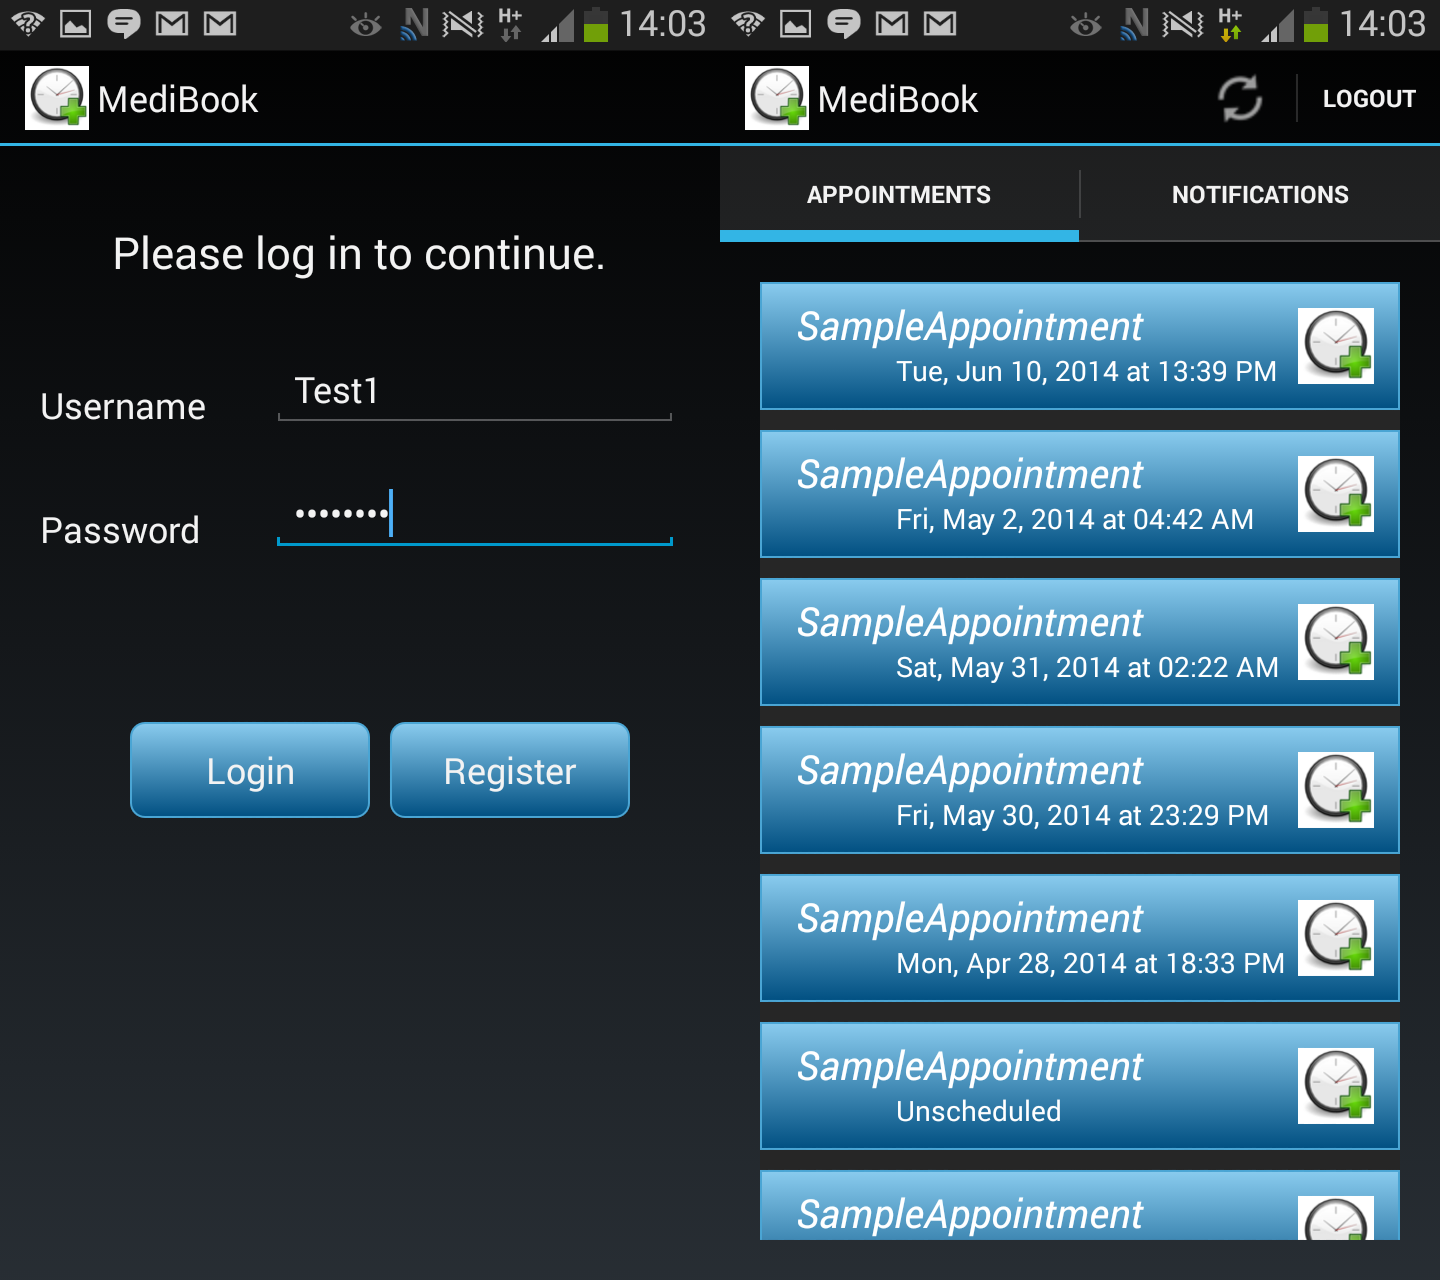
\includegraphics[width=\textwidth,height=\textheight,keepaspectratio]{Figures/screens/HomeLoginScreen.png}
		\rule{35em}{0.5pt}
	\caption[Login Screen (Left), Home Screen (Right)]{Login Screen (Left), Home Screen (Right)}
	\label{fig:loginhomescreen}
\end{figure}

\begin{figure}[htbp]
	\centering
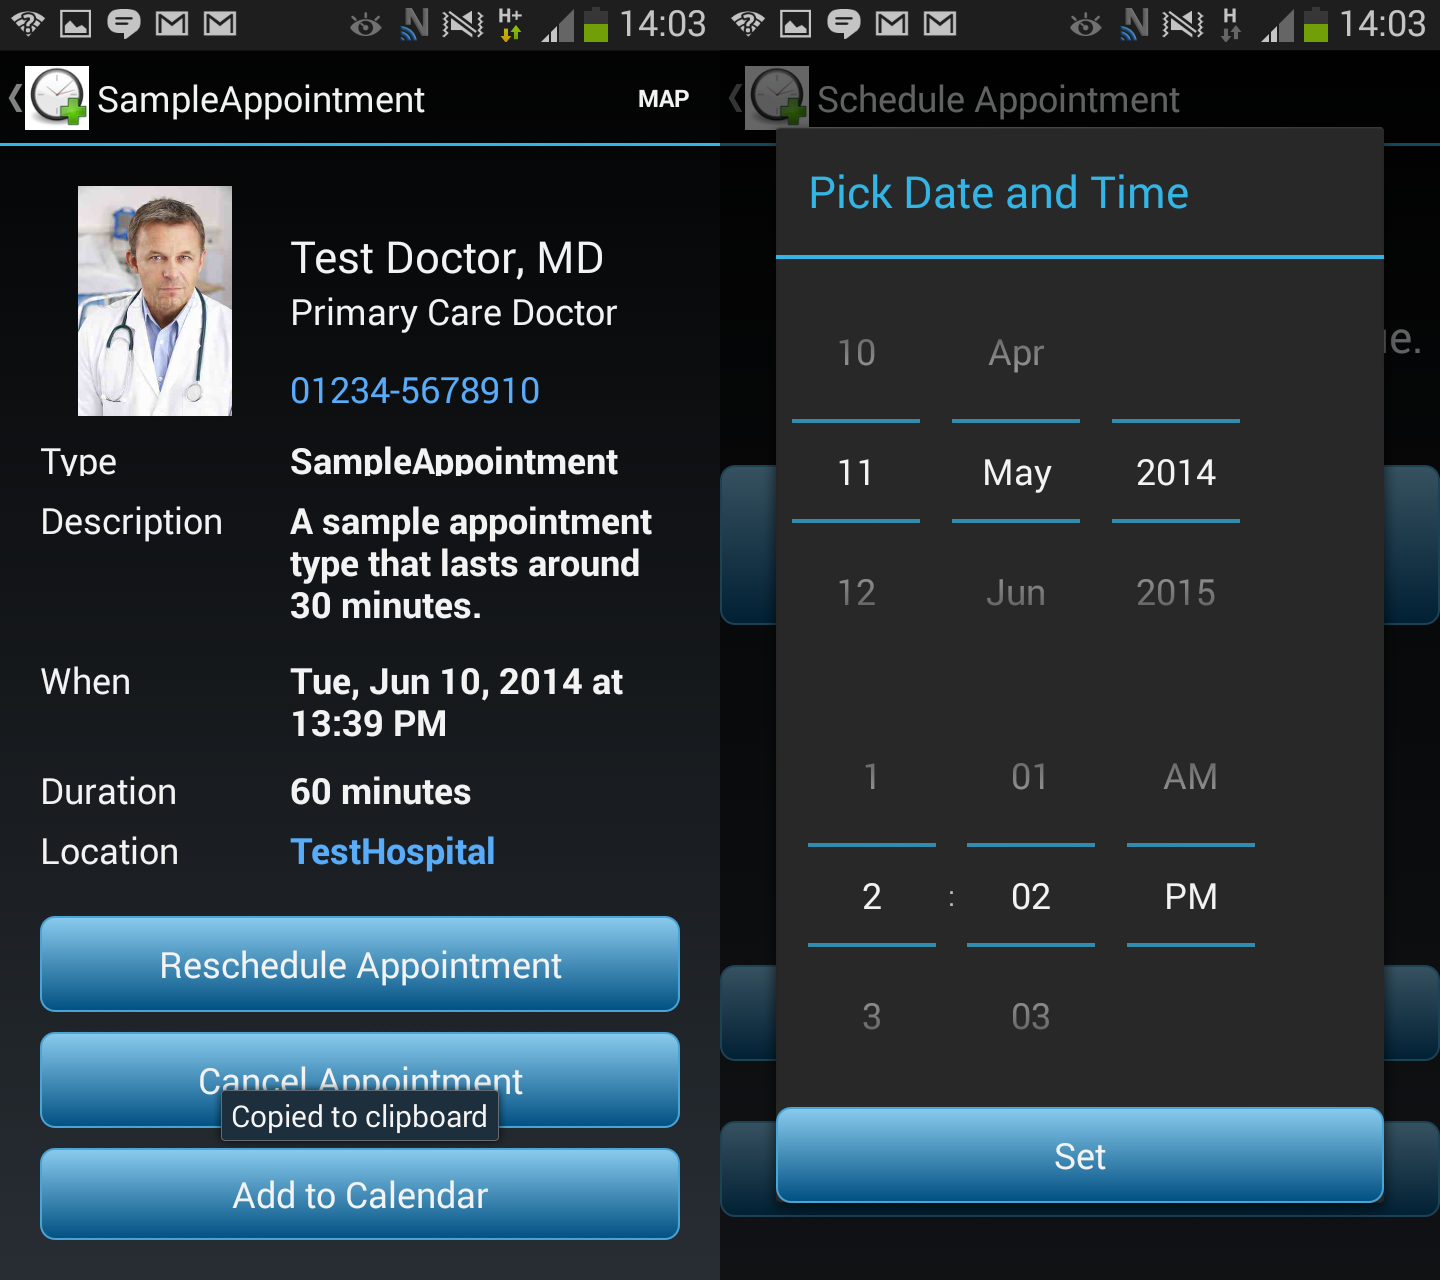
\includegraphics[width=\textwidth,height=\textheight,keepaspectratio]{Figures/screens/AppointmentScheduleScreen.png}
		\rule{35em}{0.5pt}
	\caption[Appointment Information Screen (Left), Appointment Time Picker Screen (Right)]{Appointment Information Screen (Left), Appointment Time Picker Screen (Right)}
	\label{fig:appointmentschedulescreen}
\end{figure}

\begin{figure}[htbp]
	\centering
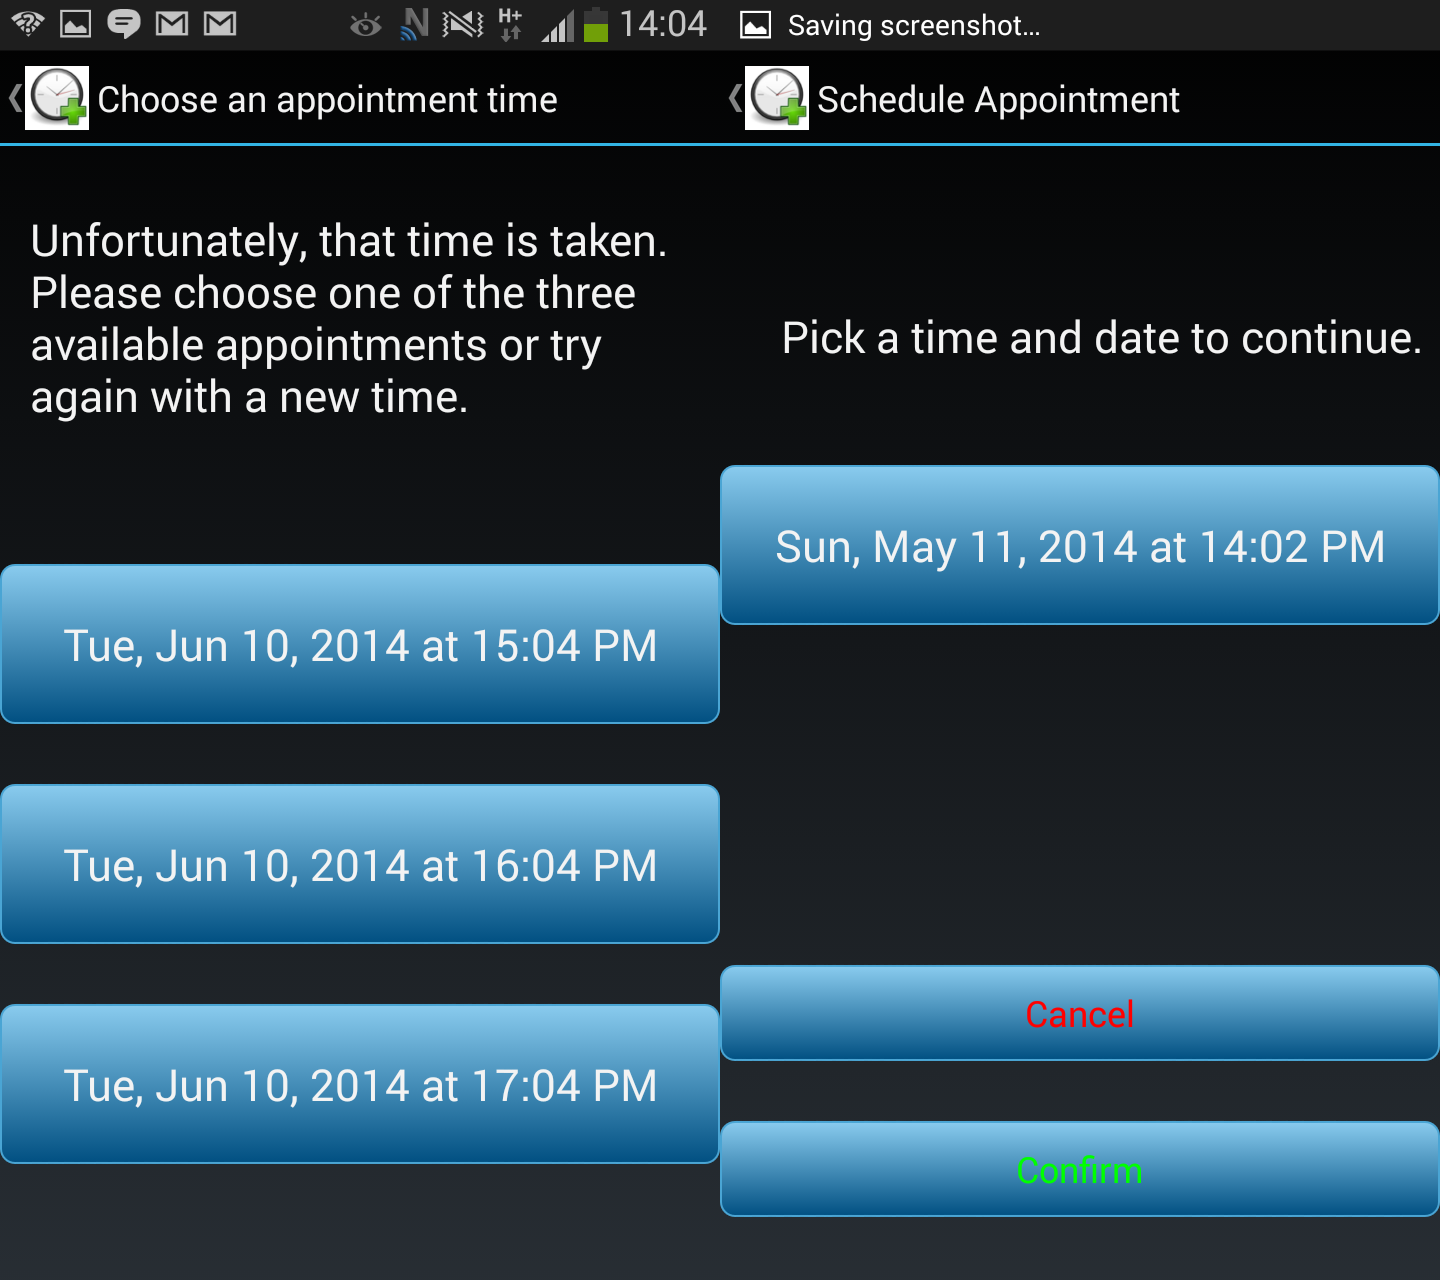
\includegraphics[width=\textwidth,height=\textheight,keepaspectratio]{Figures/screens/ConfirmScheduleScreen.png}
		\rule{35em}{0.5pt}
	\caption[Conflicting Appointment Screen (Left), Confirm Appointment Time Screen (Right)]{Conflicting Appointment Screen (Left), Confirm Appointment Time Screen (Right)}
	\label{fig:conflictappointscreen}
\end{figure}




\addtocontents{toc}{\vspace{2em}} % Add a gap in the Contents, for aesthetics

\backmatter

%----------------------------------------------------------------------------------------
%	BIBLIOGRAPHY
%----------------------------------------------------------------------------------------

\label{Bibliography}

\lhead{\emph{Bibliography}} % Change the page header to say "Bibliography"

\bibliographystyle{unsrtnat} % Use the "unsrtnat" BibTeX style for formatting the Bibliography

\bibliography{Bibliography} % The references (bibliography) information are stored in the file named "Bibliography.bib"

\end{document}  